\chapter{Zweite Methode} \label{cha:Zweite Methode}

In diesem Kapitel wird die Realisierung des zweiten Verfahrens eingegangen werden. Die Bildregistrierung wird zuerst im Detail gegeben. Anschließen läuft die Differenzbild Optimierung und die benötigte Bildverarbeitung. QR Muster Detektion werden schließlich erläutert. Zur Implementierung dieses Verfahrens wird Matlab unter der Lizenz TU Dortmund verwendet.

\section{Allgemeine Struktur} 

Dieses Verfahren verwendet die Charakteristiken der Datenmodulation des DaViD Systems, d.h. an jedem Eck des Datenebene ein QR Muster hinzu und dann mit den Daten zusammen hinter dem Bild moduliert. Am Empfängen nach einige Operationen   wird QR Muster mit die in diese Kapitel vorstellte Verfahren detektiert und schließlich bestimmt der Modulationsbereich. Diese Methode löst effektiv den unschönen Effekt, der das QR-Modul direkt zum Bild hinzugefügt wird, und kann das Problem günstiger und effektiver durch die QR-Mustereigenschaft lösen. Abbildung \ref{fig:Strukturdiagramm} zeigt die Strukturdiagramm dieses Verfahrens.

\begin{figure}[H]
 \centering 
 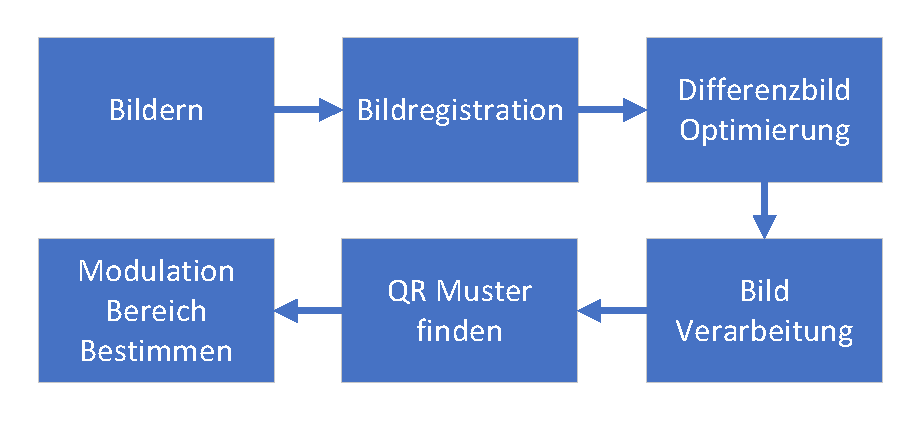
\includegraphics[keepaspectratio,width=1.0\textwidth]{images/3_Ersteverfahren/Strukturdiagramm.pdf}
 \caption{Strukturdiagramm}
 \label{fig:Strukturdiagramm}
\end{figure}

Das Objekt, das mit dieser Methode bearbeitet wird, ist die aus einer spezifischen Handy App stammte Bildern. Diese App wurde speziell für das DaVid-System entwickelt und erstellt eine Reihe von Bildern bei jeder Aufnahme. In Allgemeiner wird die Kamera bei der Aufnahme in der Hand gehalten. Aufgrund von Handschütteln während des Aufnahme werden eine leichte Verschiebung zwischen den Bildern besteht. Um dieses Problem zu lösen, nehmen eine Bildregistrierung Operation, die zwei Bilder in dasselbe Koordinatensystem konvertiert. Zuerst durch Merkmalserkennung überprüfen die Merkmal der Bildern. Dann die entsprechenden Punkte zwischen den beiden Bilder werden durch Merkmalsextraktion und Merkmalanpassung erhalten. Hier braucht ein \gls{ransac} Algorithmus, um die falschen Korrespondentpunkt zu beseitigen und die Genauigkeit zu verbessern. Aus dem Kameramodell wird dann ein mathematisches Transformations Modell zwischen den entsprechenden Punkten in den beiden Bildern erstellt. Hier bemerkt, der Prozess des Lösung dieser Transformationsmodell kann als ein nichtlineares Optimierungsproblem angesehen werden. Durch Lösung dieses Problems kann die Transformationsmatrix erhalten werden. In diesen Arbeit wählen das erste Bild immer als Referenzbild aus und nehemn einen Bildregistrierung nacheinander mit anderen Bildern. Danach bekommen eine Reihe Bilder, die in dasselbe Koordinatensystem umgewandelt. Auswälen je zwei Bilder und subtrahieren, dann erhalten eine Reihe Differenzbildern. Um die folgend Detektion zu vereinfachen, machen eine Optimierungsoperation mit der Hilfe der geometrischen Eigenschaft des QR Musters und dann erstellen ein detektierendes Bild. Anschließen eine Reihe von Bildverarbeitung bzw. Binarisierung, Medianfilter, Morphologie Operation wird behandelt. Dadurch können die kleine Punkte und Lücken, die durch Rauschen und Fehler verursacht werden, entfernt werden. Schließlich wird es durch die Charakteristik des QR Musters, das Breiteverhältnis $1:1:3:1:1$ beträgt, um QR Muster zu detektieren. Also bestimmen die Modulationsbereich. Die Flussdiagramm wird in Abbildung \ref{fig:Flussdiagramm der Methode} gezeigt. Die Details jedes Teils werden in den folgenden Abschnitten beschrieben.

\begin{figure}[H]
 \centering 
 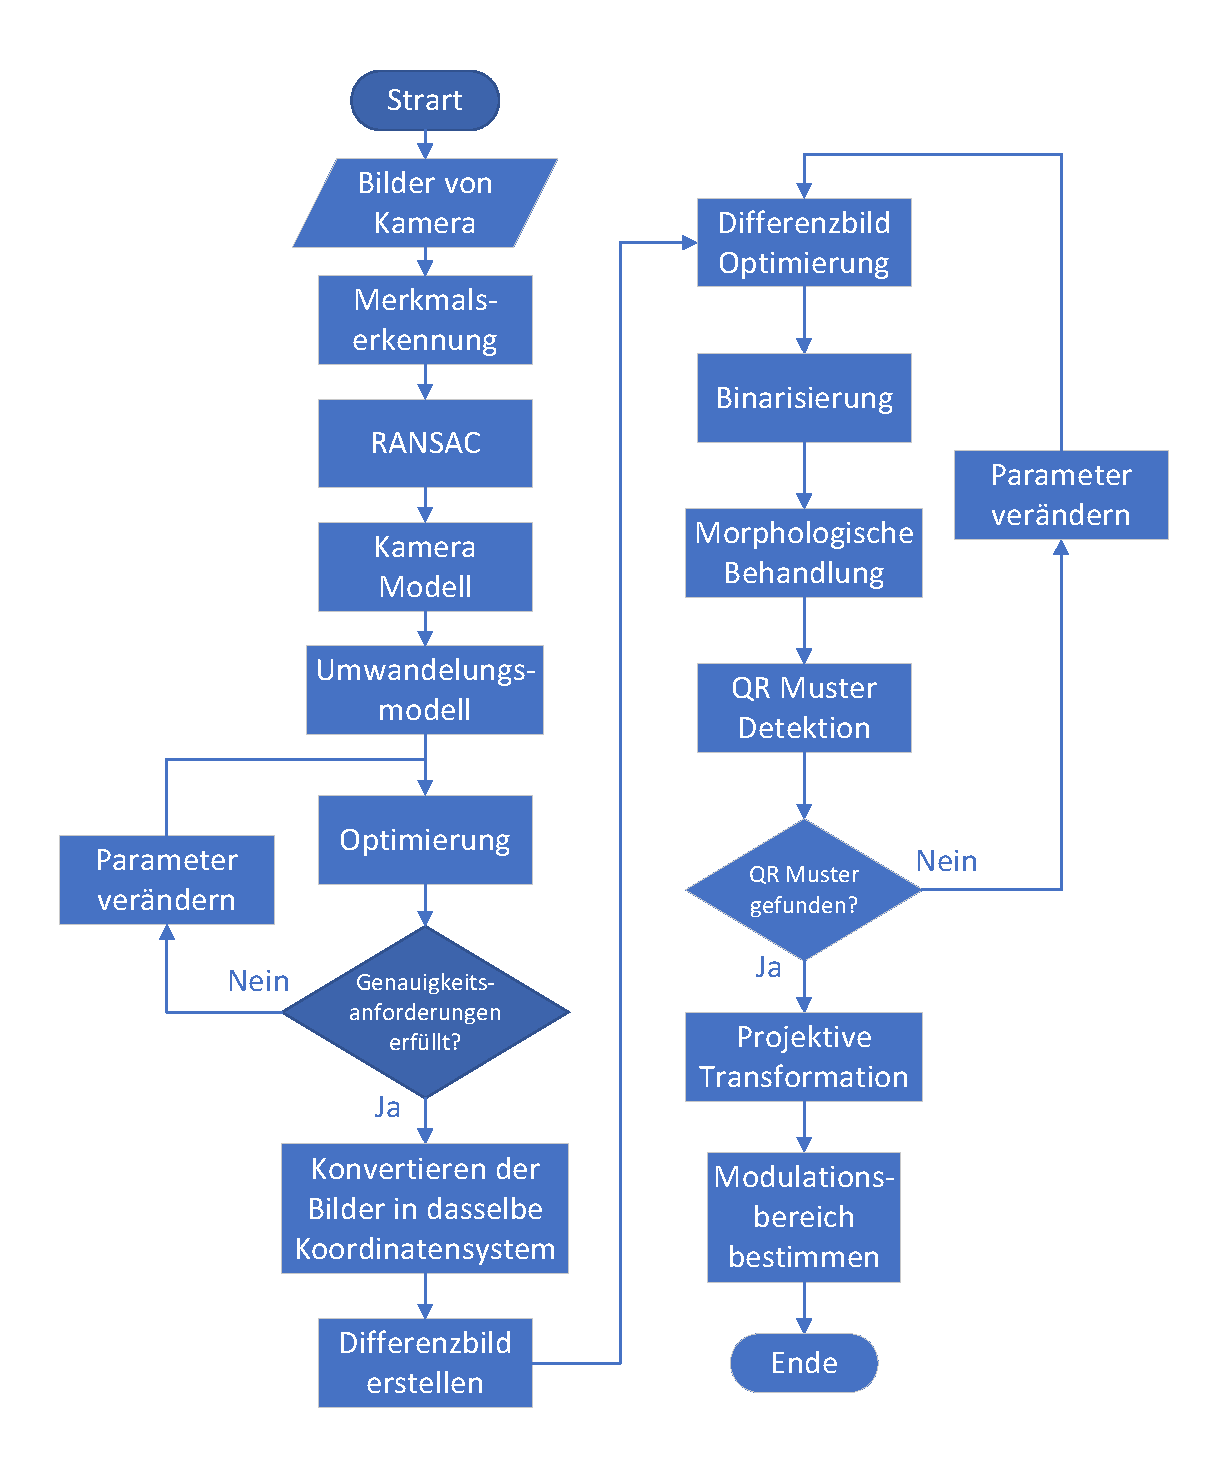
\includegraphics[keepaspectratio,width=1.0\textwidth]{images/3_Ersteverfahren/Flussdiagrammsum.pdf}
 \caption{Flussdiagramm der Methode}
 \label{fig:Flussdiagramm der Methode}
\end{figure}

\section{Bildregistrierung} 

Annehmen eine Szene, wenn eine Rhein Fotos mit einer Handheld-Kamera aufnehmen, kommt es aufgrund von Handbewegungen zu einer leichten Verschiebung zwischen den beiden benachbarten Fotos. Wenn Sie diese Fotos abziehen, um Differenzbild zu erhalten, wird der Ergebnisse sehr schlecht sein. Um diese Problem zu lösen, wird hier Bildregistrierung eingeführt. Ein Flussdiagramm der Bildregistrierung wird in Abbildung 4.2 gezeigt. 

\begin{figure}[H]
 \centering 
 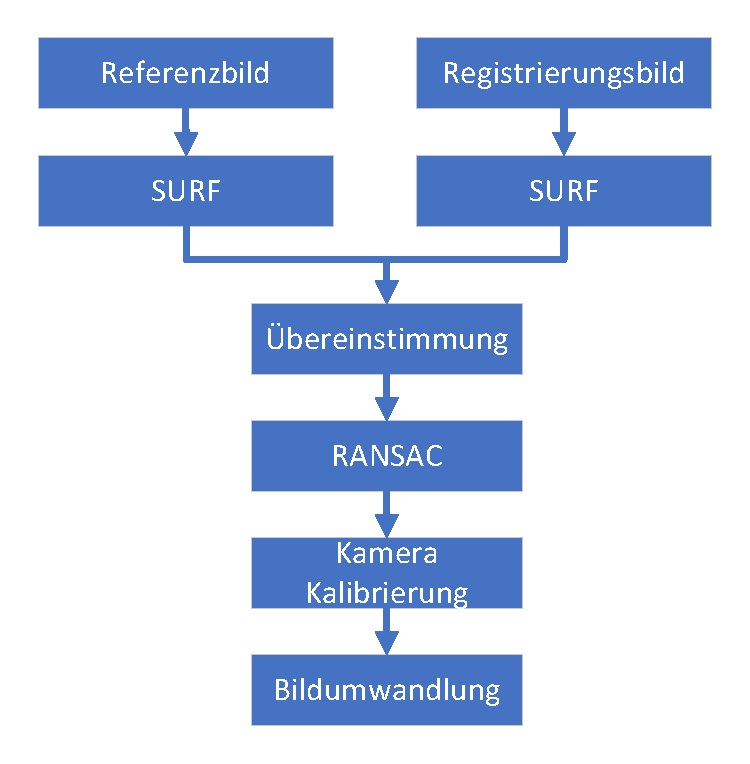
\includegraphics[keepaspectratio,width=0.6\textwidth]{images/3_Ersteverfahren/Bildregistration.pdf}
 \caption{Flussdiagramm der Bildregistrierung}
 \label{fig:Bildregistrierung}
\end{figure}

\subsection{SURF}
In jedem Bild gibt es eindeutige Pixelwertpunkte, d.h. Merkmalspunkte dieses Bildes. Um die Bilder in dasselbe Koordinatensystem zu transformieren, müssen diese Merkmalspunkte erkennt und analysiert werden. Deswegen ist das Verfahren besonders wichtig, indem die Merkmalspunkte eines Bilds definieren und finden. Um diese Problem zu lösen, wird das Konzept der Merkmalserkennung eingeführt. Die wird oft in Computer Vision und Bildverarbeitung Bereichen verwendet. Die Merkmalserkennung umfasst Verfahren zum Berechnen von Abstraktionen von Bildinformationen und zum Treffen lokaler Entscheidungen an jedem Bildpunkt, ob es an diesem Punkt ein Bildmerkmal eines bestimmten Typs gibt oder nicht. Einige typische Merkmalserkennungen sind wie z.b. Kante Detektion, Ecke Detektion, Tropfen Detektion und so weiter.

Hier in dieser Arbeite lass das SURF \cite{Surf} nutzen. 
Das ist ein patentierter lokaler Merkmal-Detektor und Deskriptor und kann für Aufgaben wie Objekterkennung, Bildregistrierung, Klassifizierung oder 3D-Rekonstruktion verwendet werden. \cite{Surf} Merkmalserkennungen ist eine verbesserte Version von SIFT Merkmalserkennungen, die Haar-Wavelet verwendet, um die Gradientenoperation in der SIFT-Methode anzunähern und gleichzeitig verwendet eine Integralgraph-Technik für schnelle Berechnungen. Die Faltung bezieht sich nur auf das vorherige Bild, mit Erhöhung der Größe des Bildkerns können das Heruntertaktung-Verfahren realisiert werden. Die Geschwindigkeit von SURF ist 3-7 mal die von SIFT mit der in den meisten Fällen entspricht   Leistung von SIFT. Daher wurde es in vielen Anwendungen eingesetzt, insbesondere in Anwendungen, in denen die Laufzeitanforderungen hoch sind. 

Der Verläuf einer SURF Merkmalserkennung ist wie flogend:

$\bullet$ \textbf{Aufbau einer hessischen Matrix.}\\
Die Hesse-Matrix stellt den Kern des SURF Algorithmus dar. Zur Vereinfachung der Operation wird die Funktion f (z, y) angenommen, dass die Hesse-Matrix H setzt sich aus Funktionen und partiellen Ableitungen zusammen:

\begin{equation}
   \mathcal{H}(f(x,y)) = \begin{bmatrix}
   \frac{\partial^{2}f}{\partial x^{2}} & \frac{\partial^{2}f}{\partial x \cdot \partial y} \\
   \frac{\partial^{2}f}{\partial x \cdot \partial y} & \frac{\partial^{2}f}{\partial y^{2}} \\   
   \end{bmatrix}
\end{equation}

 Diskriminante der H-Matrix läuft:
 
\begin{equation}
   \det(\mathcal{H}) = \frac{\partial^{2}f}{\partial x^{2}} \cdot \frac{\partial^{2}f}{\partial y^{2}} - (\frac{\partial^{2}f}{\partial x \cdot \partial y})^2  
\end{equation}

Der Wert der Diskriminante ist der Eigenwert der H-Matrix. Durch dessen positiven und negativen wird bestimmt, ob der Punkt ein Extrempunkt ist oder nicht. Im SURF Algorithmus wird das Bildpixel $l(x,y)$ anstelle des Funktionswertes $f(x,y)$ verwendet. Nutzen eine Zweite-Order Gaussian Function als Filter. Die zweiten Partielle Ableitungen können durch Faltung zwischen bestimmten Kernen berechnet werden. Dadurch können die Werte der drei Matrixelemente der H-Matrix auch berechnet werden, nämlich die H-Matrix berechnet:

\begin{equation}
\begin{split}
   &\mathcal{H}(\textbf{x},\sigma) = \begin{bmatrix}
   L_{xx}(\textbf{x},\sigma)\ L_{xy}(\textbf{x},\sigma) \\
   L_{xy}(\textbf{x},\sigma)\ L_{yy}(\textbf{x},\sigma)
   \end{bmatrix} \\   
   &L(\textbf{x},\sigma) = G(\sigma)*I(\textbf{x}) \\  
   &G(\sigma) = \frac{\partial^{2}g(\sigma)}{\partial x^{2}}      
\end{split}
\end{equation}


Hier $L_{xx}(\textbf{x},\sigma)$ bedeutet die Faltung der zweiter Gaussian Ableitung $G(\sigma)$ mit dem Bild I in Punkt $\textbf{x}$(x,y), ähnlich für $L_{xy}(\textbf{x},\sigma)$ und $L_{yy}(\textbf{x},\sigma)$. Auf diese Weise kann der Wert der Determinante für jedes Pixel in dem Bild berechnet werden, und dieser Wert kann verwendet werden, um den Merkmalspunkt zu feststellen.
Zur einfacheren Anwendung schlägt Herbert Bay\cite{Surf} vor, L mit einer Approximation ersetzen. Um den Fehler zwischen dem genauen Wert und der Approximation auszugleichen, kann die H-Matrix-Diskriminante wie folgt ausgedrückt werden:

\begin{equation}
   \det(\mathcal{H}_{Approx}) = D_{xx}D_{yy} - (0.9D_{xy})^2  
\end{equation}
\\
$\bullet$ \textbf{Erstellen Maßstab Raum}\\
Der Maßstabsraum $L(\textbf{x},\sigma)$ des Bildes ist die Darstellung dieses Bildes bei unterschiedlichen Auflösungen(Skalierung). Im Bereich der Computer Vision wird der Maßstabsraum symbolisch als Bildpyramide ausgedrückt, wobei die Eingangsbildfunktion wiederholt mit dem Kern der Gaußschen Funktion gefaltet und wiederholt unterabgetastet wird. Diese Methode wird hauptsächlich für die Implementierung des SIFT Algorithmus verwendet. Jede Bildschicht hängt jedoch von der vorherigen Bildschicht ab, und das Bild muss in der Größe angepasst werden. Daher hat diese Berechnungsmethode eine große Kosten in Berechnung. Im Vergleich dazu ist es in SURF durch die Erhöhung der Größe des Bildkerns. Diese ist ein Unterschied zwischen dem SIFT Algorithmus und dem SURF Algorithmus bei der Verwendung des Pyramidenprinzips.
Der Algorithmus ermöglicht, dass mehrere Bilder des Maßstabsraums gleichzeitig verarbeitet werden, ohne dass das Bild unterabgetastet wird, wodurch die Leistung des Algorithmus verbessert wird. Das linke Bild in Abbildung 4.3 ist eine Pyramidenstruktur, die auf herkömmliche Weise erstellt wird, die Größe des Bildes wird geändert, und die Operation wird die Unterebene  unter Verwendung der Gaußschen Funktion wiederholt glätten. Der Surf Algorithmus auf der rechten Seite in Abbildung 4.3 behält das ursprüngliche Bild unverändert und ändert nur die Filtergröße.

\begin{figure}[htb]
 \centering 
 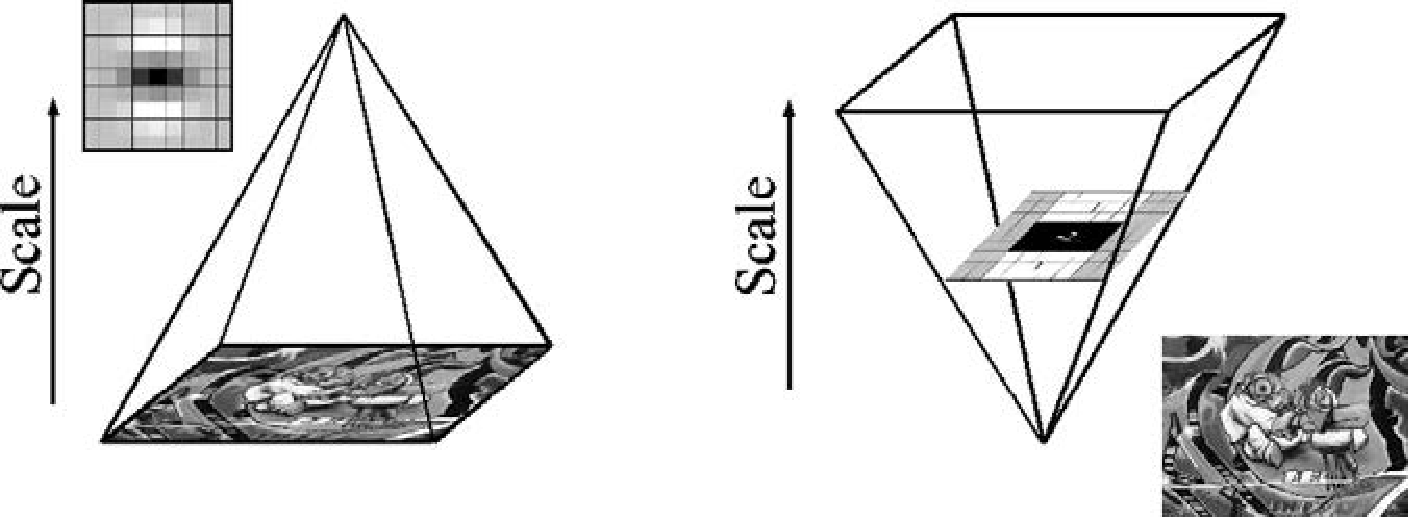
\includegraphics[keepaspectratio,width=0.8\textwidth]{images/3_Ersteverfahren/Scale_space.pdf}
 \caption{Scale space}
 \label{fig:Scale space}
\end{figure} 


$\bullet$ \textbf{Präzise Lokalisierung von Feature-Punkten}\\
Vergleichen die Größe jedes Pixel, die von der hessischen Matrix verarbeitet wird, mit die 26 Punkten in seiner drei Dimensionen Raum, wie in Abbildung 4.4 zeight. Wenn es das Maximum oder Minimum dieser 26 Punkte ist, wird es als vorläufiger Merkmalspunkt beibehalten. Das dreidimensionale lineare Interpolationsverfahren wird verwendet, um die Merkmalspunkte des Subpixel-Niveaus zu erhalten, und die Punkte, deren Werte kleiner als ein bestimmter Schwellenwert sind, werden ebenfalls entfernt.

\begin{figure}[htb]
 \centering 
 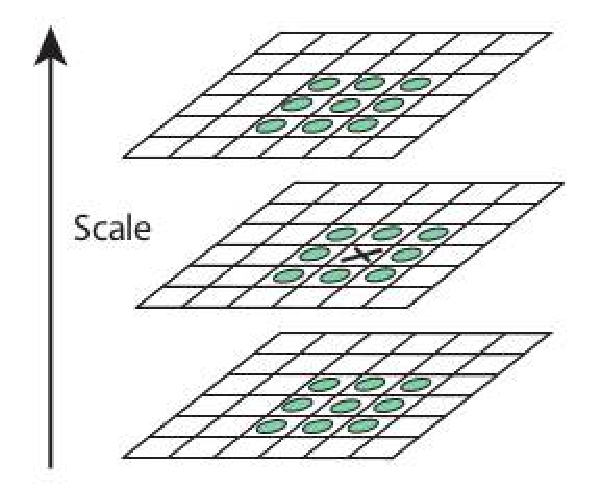
\includegraphics[keepaspectratio,width=0.4\textwidth]{images/3_Ersteverfahren/Extreme_Wert_Erkennung.pdf}
 \caption{Extreme Wert Erkennung}
 \label{fig:Extreme Wert Erkennung}
\end{figure} 


$\bullet$ \textbf{Hauptrichtungsermittlung}\\
SIFT wählt die Hauptrichtung des Merkmalspunkts unter Verwendung des Gradientenhistogramms im Merkmalspunktbereich aus. Die Richtung, in der der Bin-Wert des Histogramms der größte und oder 80\% maximale Bin-Wert  überschreitet, wird als Hauptrichtung des Merkmalspunkts genommen. Dagegen beim SURF wird das Gradientenhistogramm nicht statistiken, sondern das Harr-Wavelet-Eigenshcaft im Merkmalspunktbereich wird statistisch analysiert. Das heißt, im Bereich der Merkmalspunkt (zum Beispiel innerhalb eines Kreises mit einem Radius von 6s, wobei s der Maßstab ist, auf dem der Punkt liegt) die Summe der Horizontal-Haar-Wavelet-Merkmale und der Vertikal-Haar-Wavelet-Merkmale aller Punkte im  60-Grad-Sektor($\pi/3$) werden gezählt. Die Größe des Haar Wavelets stellt als 4s, so dass für jeden Sektor einen Wert bekommt. Dann wird 60-Grad-Sektor in einem bestimmten Intervall gedreht, schließlich lassen die Richtung des Sektors mit Maximalwert als Hauptrichtung des Merkmalspunkts nehmen. Ein schematisches Diagramm des Prozesses ist wie folgt in Abbildung 4.5.

\begin{figure}[htb]
 \centering 
 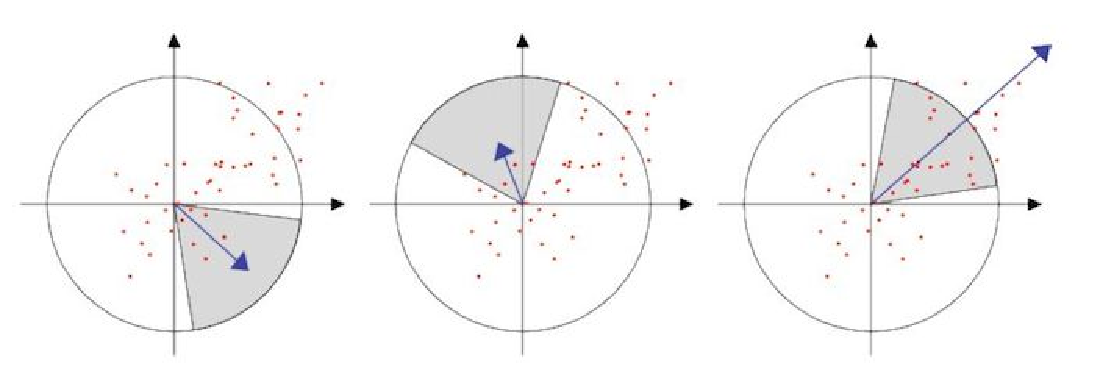
\includegraphics[keepaspectratio,width=0.8\textwidth]{images/3_Ersteverfahren/Dominante_Orientierung_Feststellen.pdf}
 \caption{Dominante Orientierung Feststellen}
 \label{fig:Dominante Orientierung Feststellen}
\end{figure} 


$\bullet$ \textbf{Merkmalspunkt Deskriptor Generierung}\\
SURF nehmen eine quadratische Rahmen um den Merkmalspunkt. Die Seite der Rahmen ist 20s (s ist die Skala, bei der der Merkmalspunkt erkannt wird). Die Richtung des Rahmens ist natürlich die Hauptrichtung, die in vorliegened Schritt erfasst wird. Die Rahmen wird dann in 16 Unterbereiche unterteilt, von denen jeder die Haar-Wavelet-Merkmale der horizontalen und vertikalen Richtungen von 25 Pixeln berechnen. Hier die horizontalen und vertikalen Richtungen sind relativ zur Hauptrichtung. Das Haar Wavelet-Merkmal ist die Summe der horizontalen Richtungswerte, die Summe der absoluten Werte in der horizontalen Richtung, die Summe der vertikalen Richtungen und die Summe der absoluten Werte in der vertikalen Richtung. Das schematisches Diagramm in Abbildung 4.6 zeigt dieses Prozesse.

\begin{figure}[htb]
 \centering 
 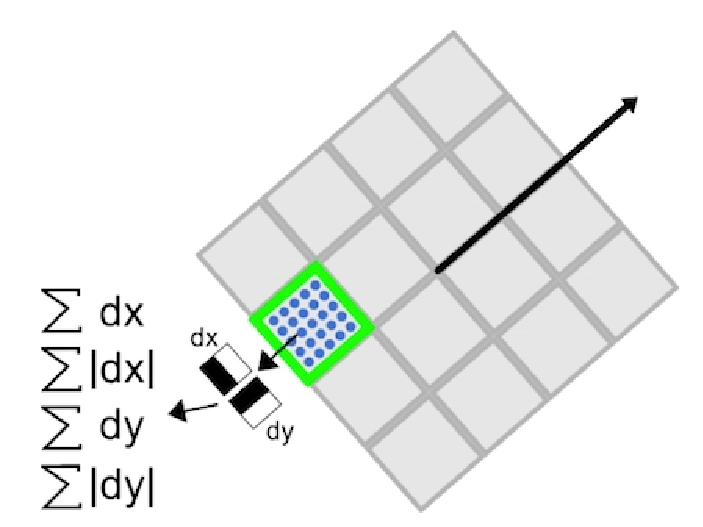
\includegraphics[keepaspectratio,width=0.5\textwidth]{images/3_Ersteverfahren/Merkmalspunkt_Deskriptor.pdf}
 \caption{Merkmalspunkt Deskriptor}
 \label{fig:Merkmalspunkt Deskriptor}
\end{figure} 

Auf diese Weise hat jeder kleine Bereich 4 Werte, so dass jeder Merkmalspunkt ein $16*4=64$ dimensionaler Vektor verfügt, der halb so klein wie Sift(128 Dimension) ist, deswegen den Anpassungsprozess beim Merkmalanpassungsprozess stark beschleunigt. Die folgende Abbildung 4.7 zeigt den Merkmalspunkt, den wir durch den SURF-Algorithmus erhalten haben.

\begin{figure}[H]
 \centering 
 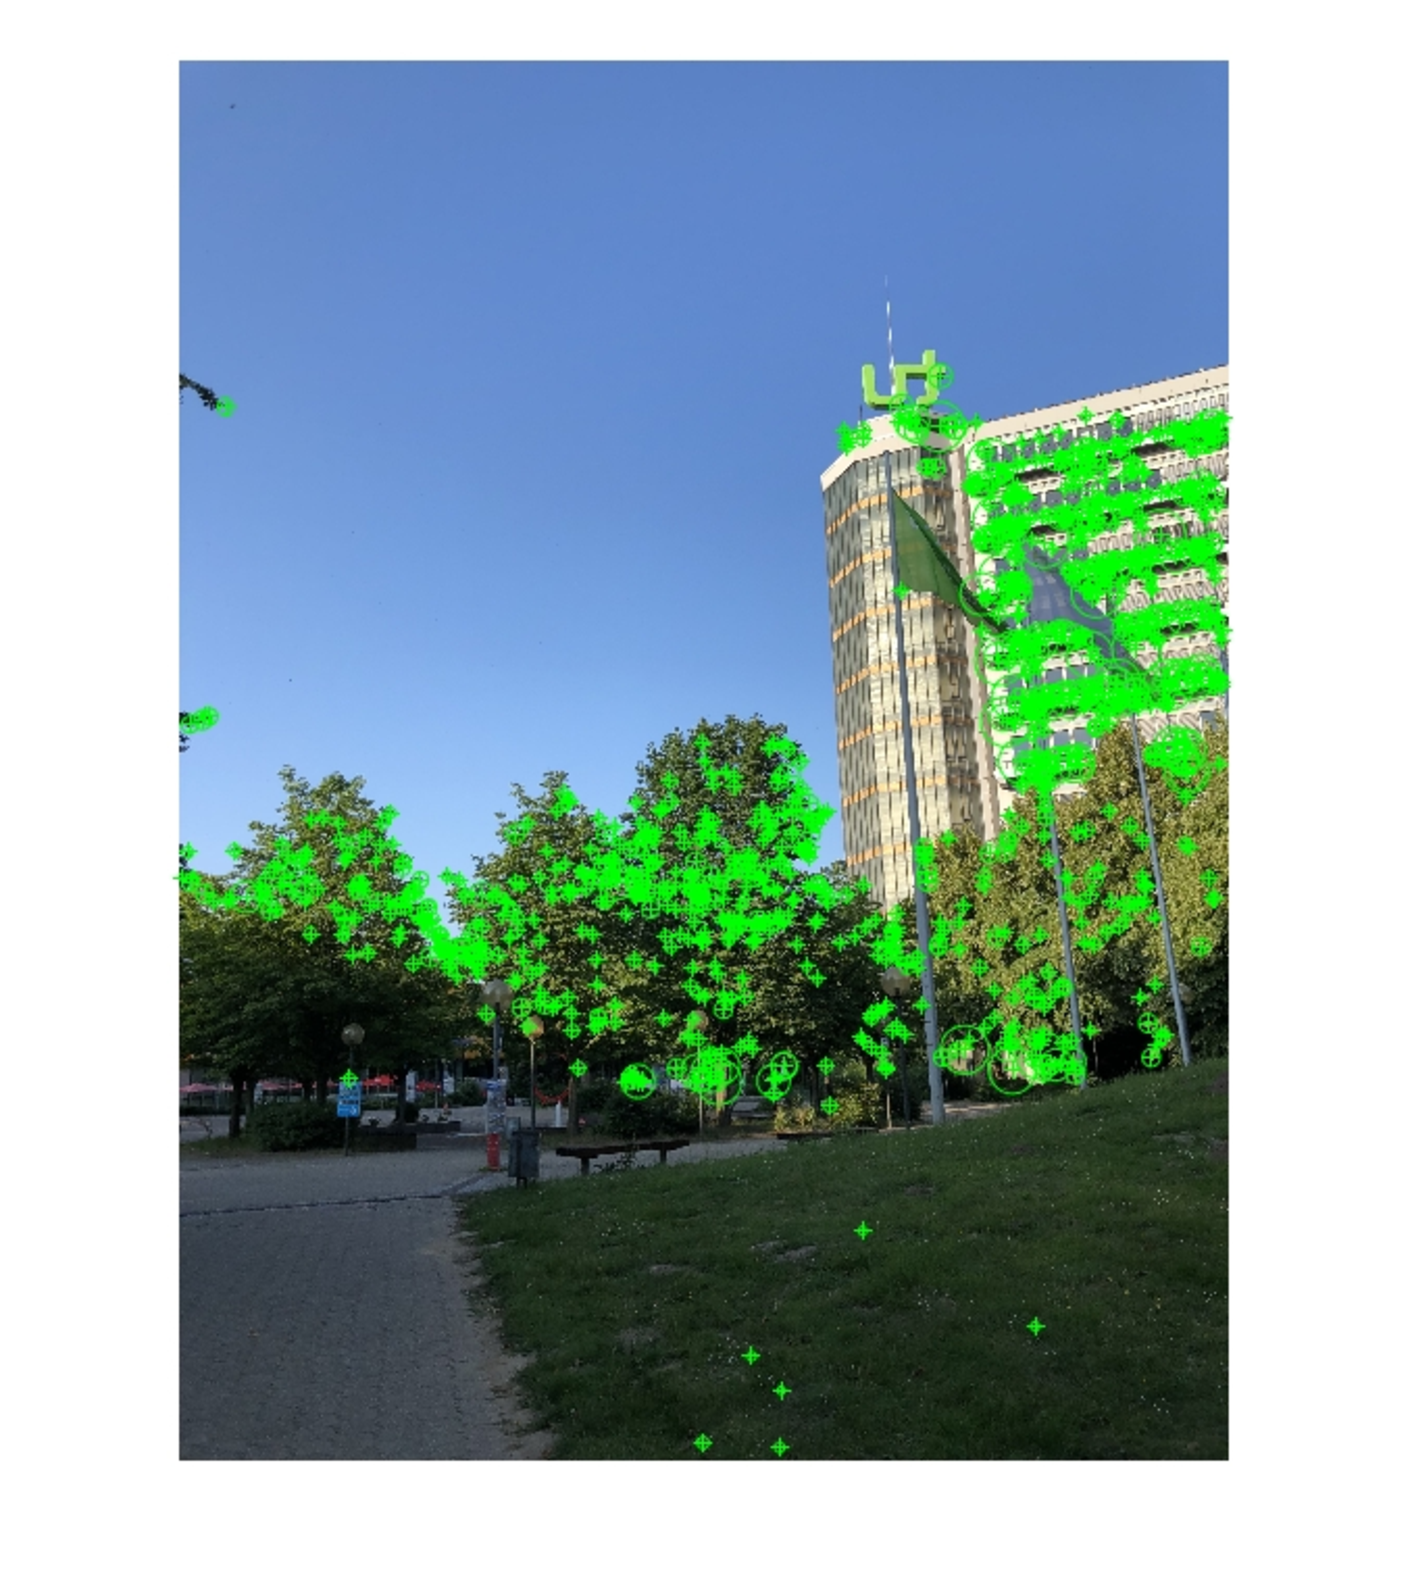
\includegraphics[keepaspectratio,width=0.8\textwidth]{images/3_Ersteverfahren/SURF_Detektion.pdf}
 \caption{SURF Merkmal}
 \label{fig:SURF Merkmal}
\end{figure} 


\subsection{RANSAC}

Nach SURF Merkmalserkennung wird die Merkmal von zwei benachbarten Bildern bekommen. Diese Merkmale werden dann mit extrahiert und abgeglichen, um entsprechende Punkte in den benachbarten zwei Bildern zu erhalten. Leider darin durch diese Operation gibt es immer noch viele fehlerhafte zusammenpassendes Paar. Deswegen wird hier \gls{ransac} eingeführt, um die falschen Punkt zu beseitigen.

RANSAC Algorithmus, der von Fischler und Bolles \cite{ransac1} vorgeschlagene im Jahr 1981, ist ein allgemeiner Parameterschätzungsansatz, um den großen Anteil von Ausreißern in den Eingabedaten zu bewältigen. Im Gegensatz zu vielen der üblichen robusten Schätzverfahren wie M-Schätzer und kleinsten Quadraten, die von der Computer Vision Community aus der Statistik-Literatur übernommen wurden, wurde RANSAC aus der Computer-Vision-Community entwickelt. 

Ein einfaches Beispiel ist in der Abbildung 4.7 dargestellt. Das Ziel besteht darin, die am besten geeignete Linie unter einer Menge von Datenpunkten zu finden. Wenn es die einfache Methode der kleinsten Quadrate verwenden ,um diese Linie zu finden, wie auf der linken Seite gezeigt, kann es leider nicht richtig finden, da die Methode der kleinsten Quadrate von alle Datenpunkte beeinflusst wird. Dagegen mit RANSAC kann das Modell nur von der inlierer Punkte berechnet werden und die Ergebnisse wie auf der rechten Seite zeigt. 

\begin{figure}[H]
 \centering 
 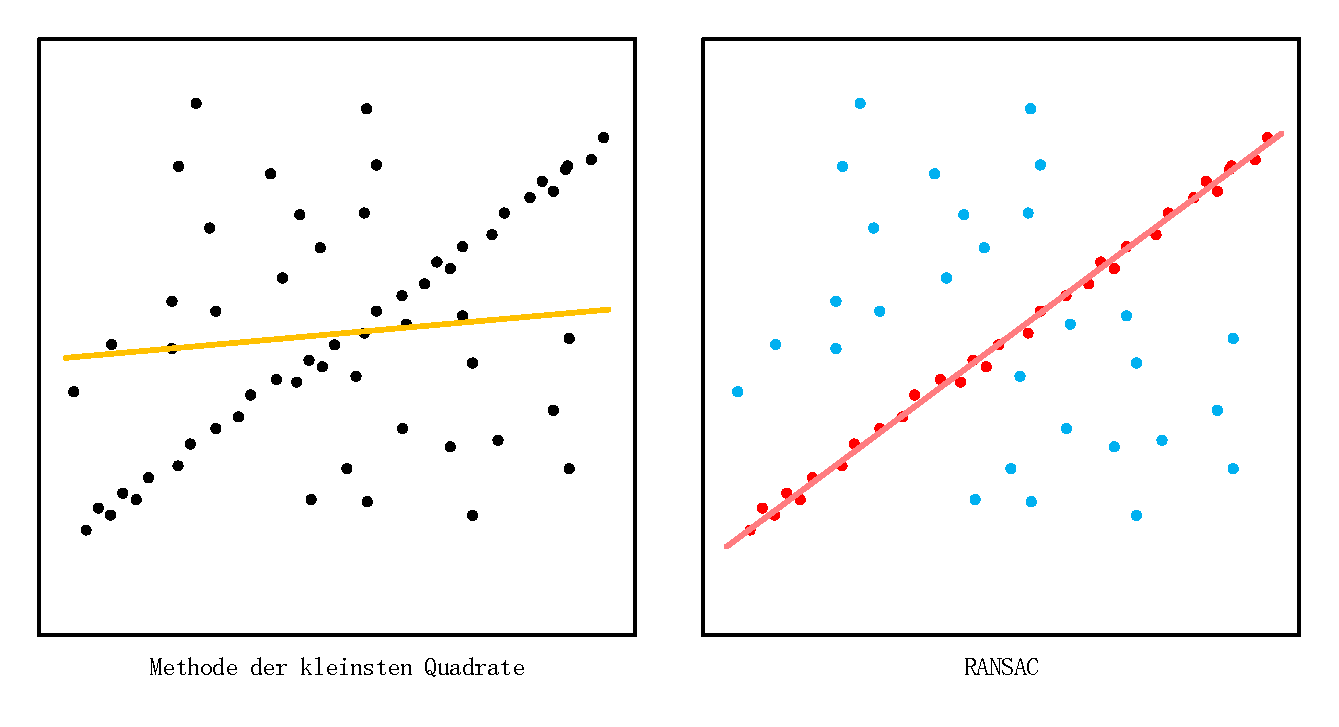
\includegraphics[keepaspectratio,width=1.0\textwidth]{images/3_Ersteverfahren/RANSAC/Linien_Detektion.pdf}
 \caption{Linien Detektion}
 \label{fig:Linien Detektion}
\end{figure} 

RANSAC ist ein Wiederholungsprobennahme Verfahren, das  durch die minimalen Anzahl von Beobachtungenpunkten (Datenpunkten) die Kandidatenlösungen generiert. Diese Datebpunkten sind die erforderlich, um die zugrunde liegenden Modellparameter zu schätzen. Darauf haben Fischler und Bolles~\cite{ransac1} hingewiesen, zur Erhalten einer anfängliche Lösung und Beschneidung der Ausreißern RANSAC Verfahren baraucht nicht so viele Daten, sondern verwendet die kleinste mögliche Menge und fährt fort, diese Menge mit eine konsistenten Datenpunkten zu vergrößern.

Der grundlegende Algorithmus ist wie folgt zusammengefasst:

\begin{itemize}
	\item Zufällig wählen die Mindestanzahl der Punkten aus, die erforderlich sind, zum Bestimmen der Modellparameter.
	\item Lösen die Parameter des Modells.
	\item Bestimmen wie viele Punkte aus der Menge aller Punkte mit einer vordefinierten Toleranz $\epsilon$ übereinstimmen
	\item Wenn der Bruchteil der Anzahl von Inlierern über die Gesamtzahl der Punkte in dem Satz einen vordefinierten Schwellenwert $\tau$ überschreitet, schätzen die Modellparameter mit allen identifizierten Inlierern und terminieren wieder.
	\item Ansonsten wiederholen die Schritte 1 bis 4 (maximal N-mal).
\end{itemize}

N bedeutet die Anzahl der Iterationen. Es wird hoch genug gewählt, um die Wahrscheinlichkeit p (normalerweise auf 0,99 gesetzt) sicherzustellen, dass mindestens eine der Gruppen von Stichproben keinen Ausreißer enthält.
Dann die Wahrscheinlichkeit, dass bei N Mal Iterationen mit erforderlich minimalen Anzahl Punkte (hier m annahmen) mindestens ein Ausreißer mit ausgewählt wird, läuft:

\begin{equation}
   1 - p = (1 - u^m)^N
\end{equation}

Hier u stellen die Wahrscheinlichkeit dar, dass jeder ausgewählte Datenpunkt ein Inlier ist. Dagegen $v = 1 - u$ heißt die Wahrscheinlichkeit, dass jeder ausgewählte Datenpunkt ein Ausreißer ist. Durch einige Gleichheitsumwandlung können die Anzahl der Iterationen ausgedrückt werden als:

\begin{equation}
   N = \frac{\log(1 - p)}{\log(1 - (1 - v)^m)}
\end{equation}

Abbildung 4.8 zeigt die passende Punkt durch Merkmalübereinstimmung mit \gls{surf} Detektion. Es ist ersichtlich, dass es viele fehlerhafte Kombinationen gibt. Dagegen durch die Anwendung von RANSAC kann dieses Problem effektiv lösen und die übereinstimmendenPunkte verfeinern, die Ergebnisse wie in Abbildung 4.9 zeigt.

\begin{figure}[H]
 \centering 
 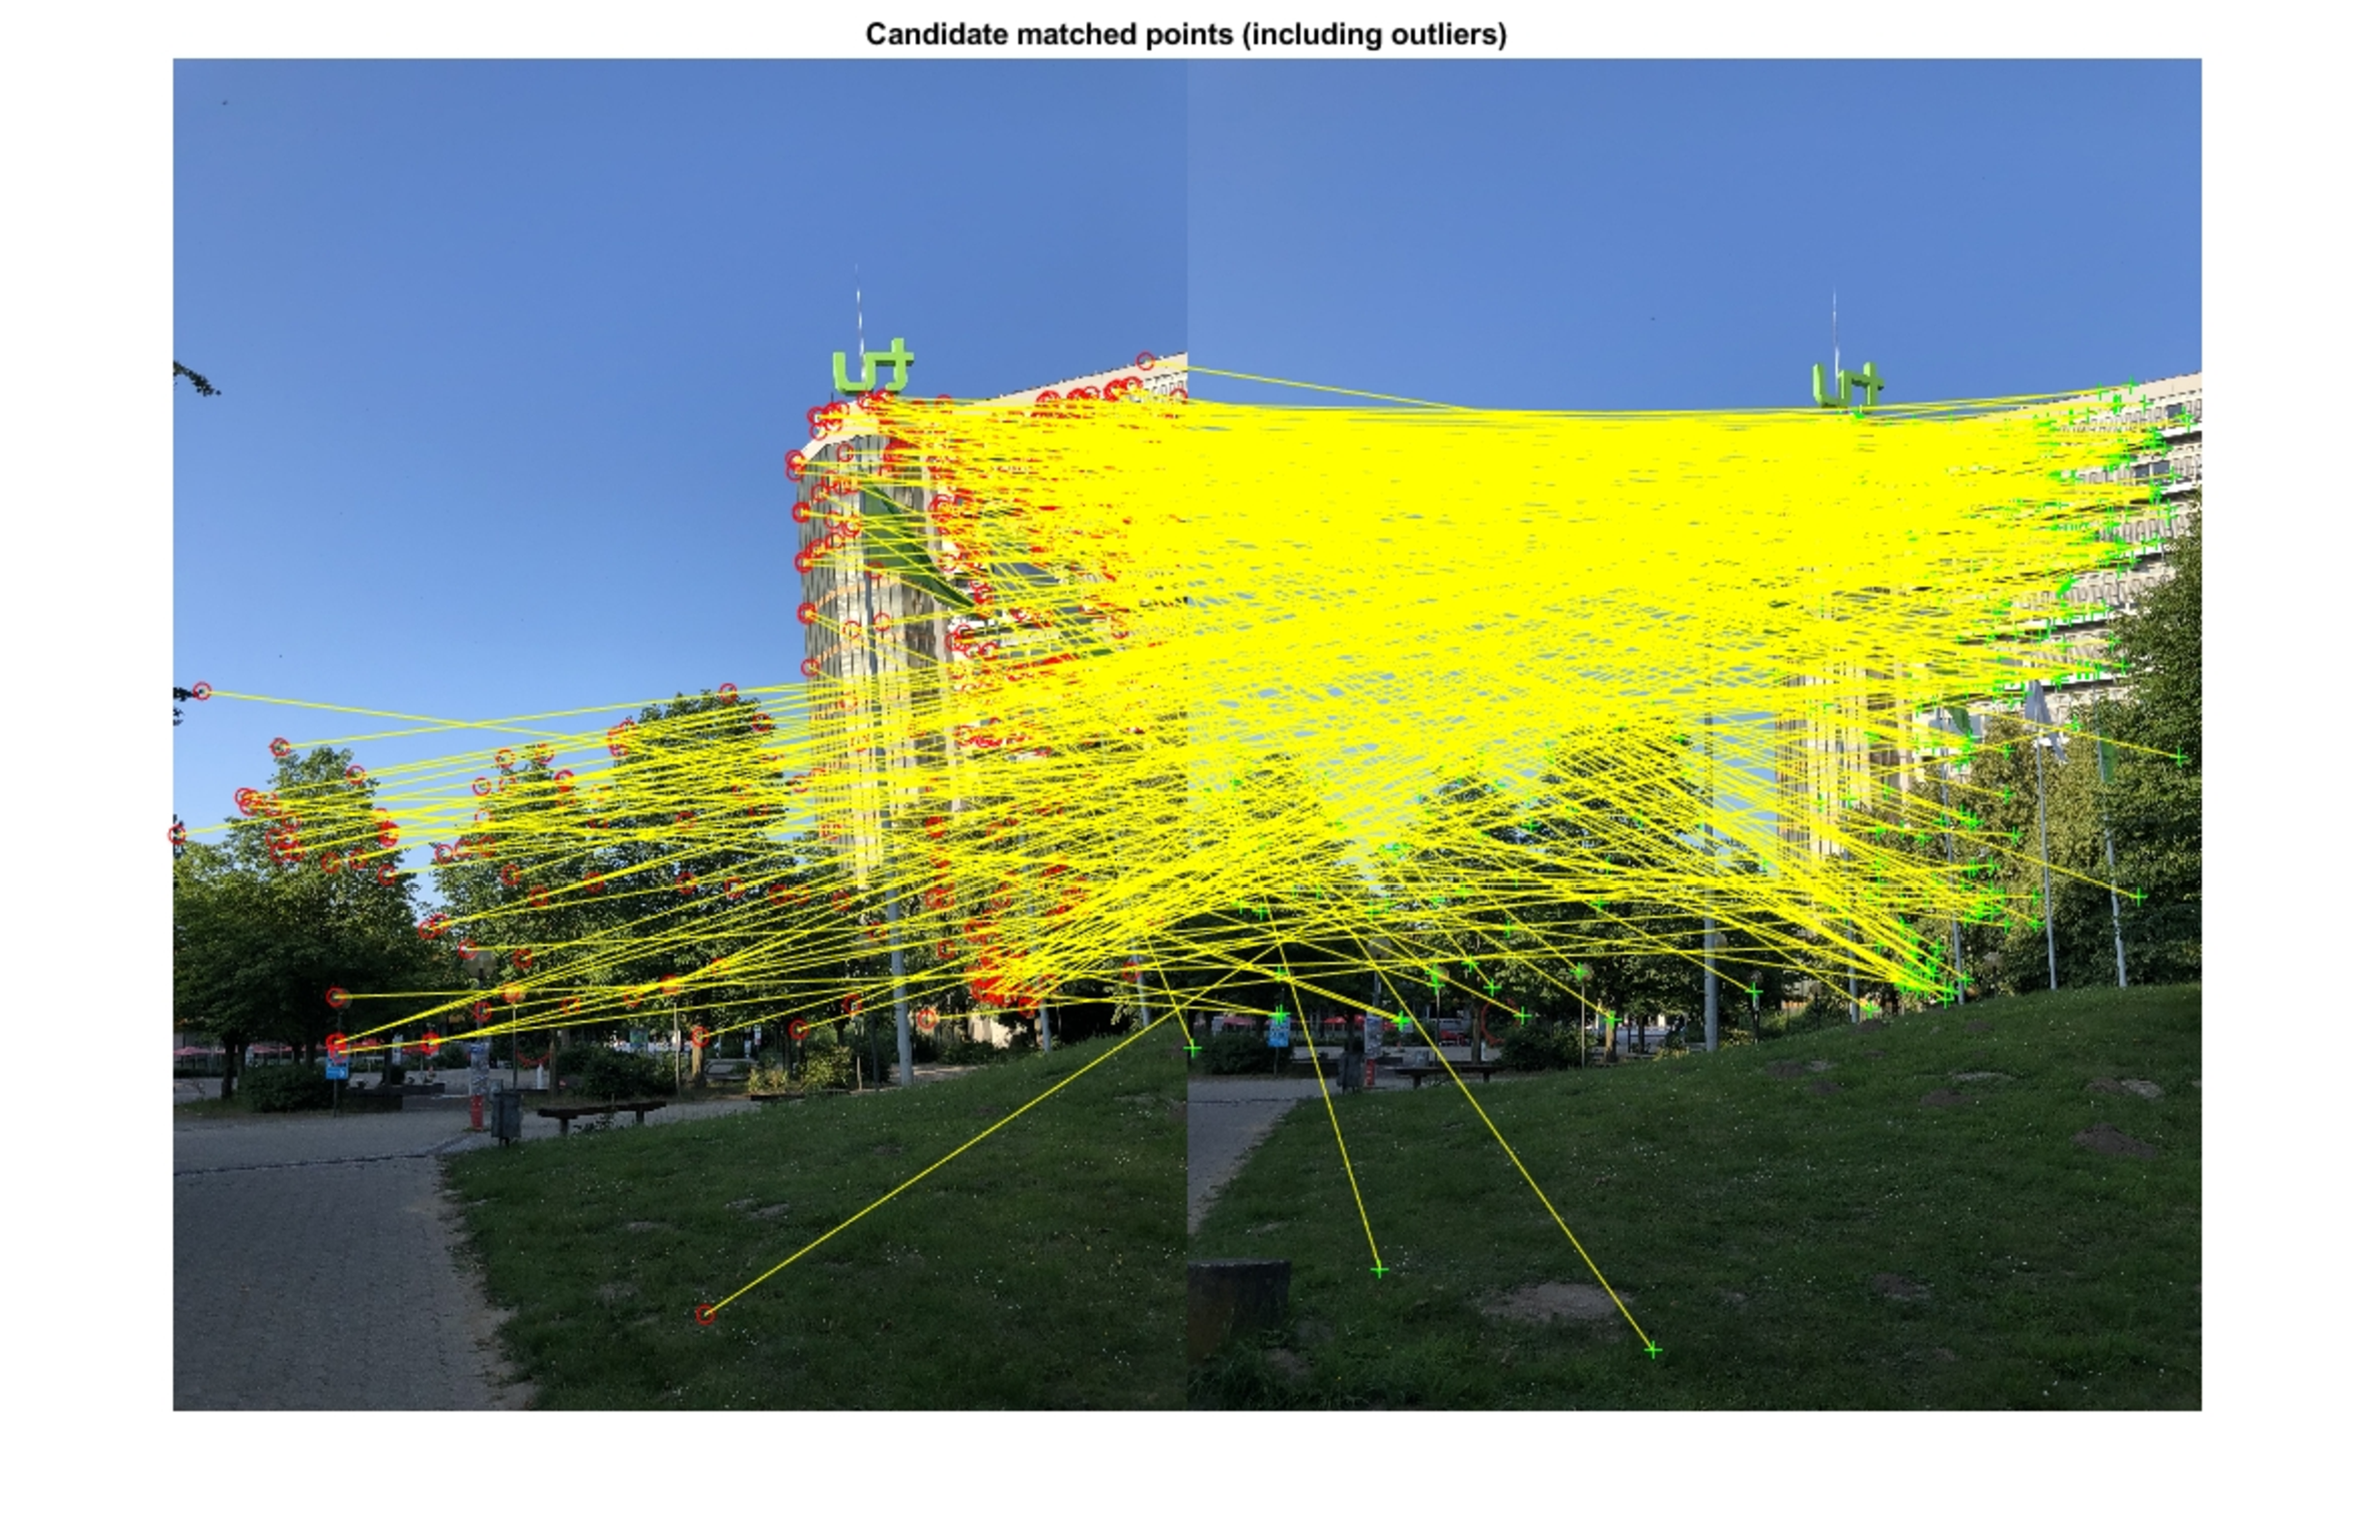
\includegraphics[keepaspectratio,width=0.9\textwidth]{images/3_Ersteverfahren/RANSAC/OhneRANSAC.pdf}
 \caption{OhneRANSAC}
 \label{fig:OhneRANSAC}
\end{figure} 

\begin{figure}[H]
 \centering 
 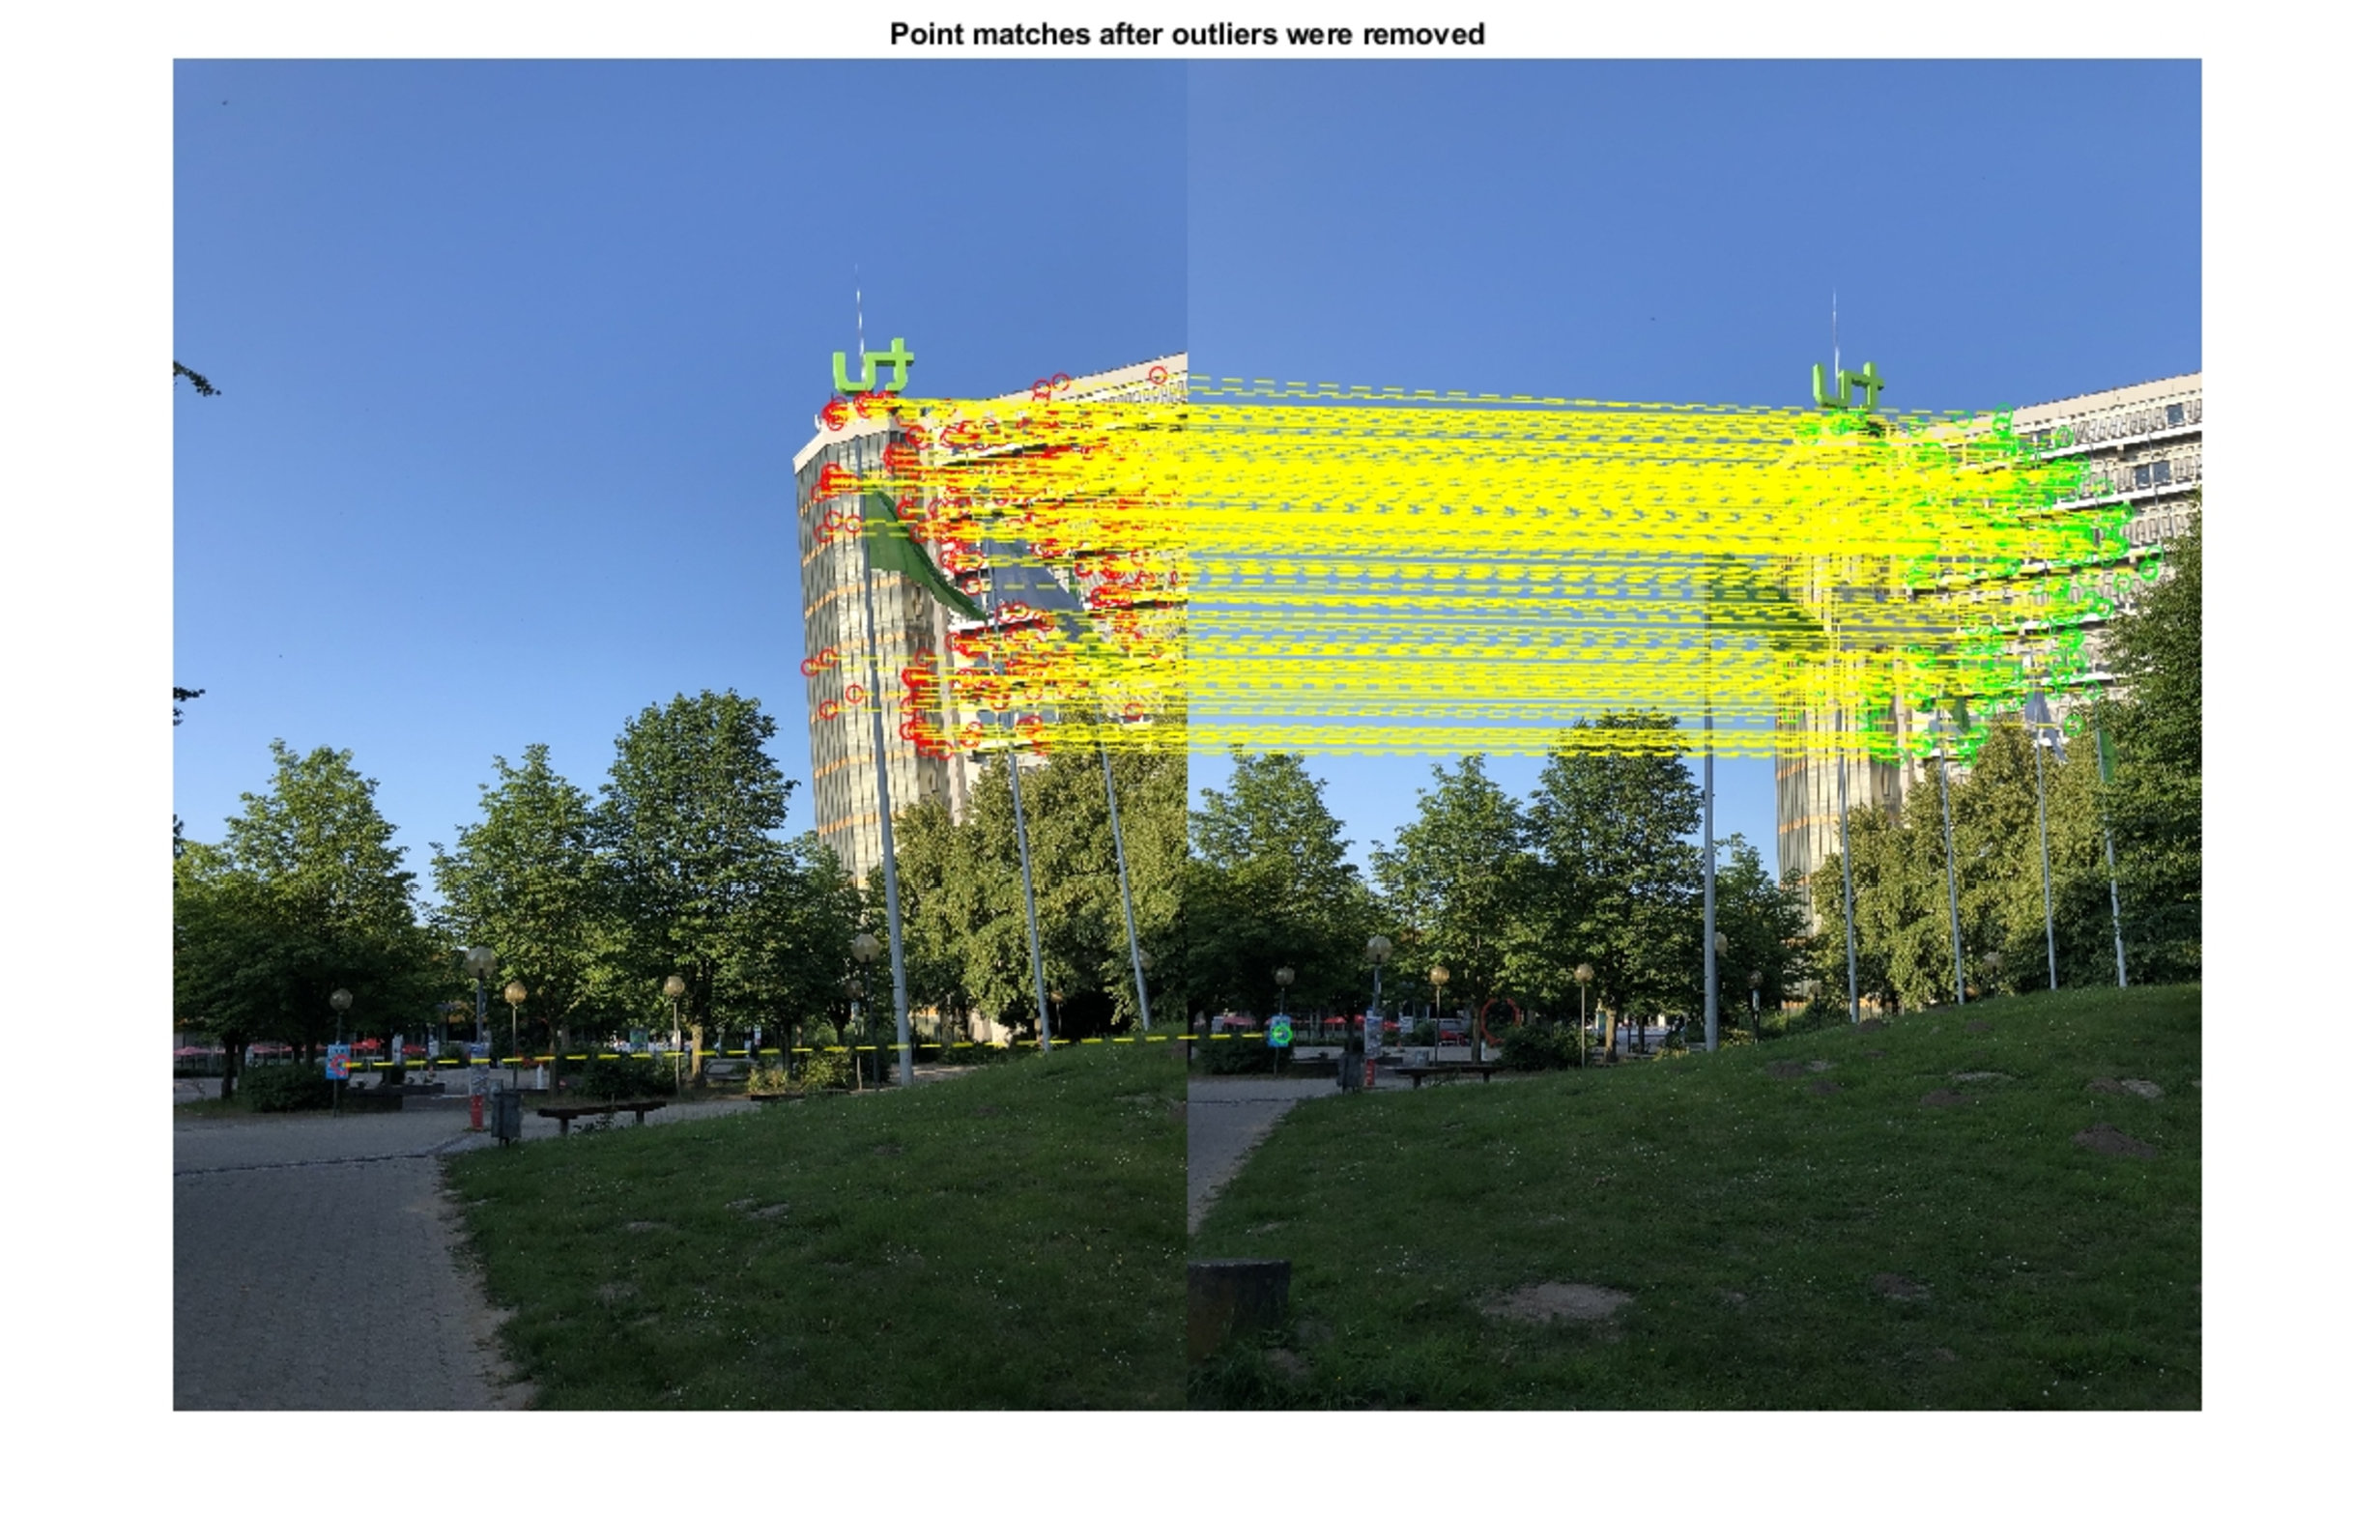
\includegraphics[keepaspectratio,width=0.9\textwidth]{images/3_Ersteverfahren/RANSAC/MitRANSAC.pdf}
 \caption{MitRANSAC}
 \label{fig:MitRANSAC}
\end{figure} 


\subsection{Bilder Umwandlung}

Wie in den vorliegend Abschnitten vorgestellt, mit Verwenden des SURF finden die übereinstimmende Punkte in aufeinanderfolgenden Bildern, anschließen durch RANSAC lassen die Ausreißer verwerfen. Das Ziel dieses Abschnitts besteht darin, das Bild in dasselbe Koordinatensystem zu konvertieren. Der erste Schritt ist, ein Kameramodell zu erstellen und dann darauf die Umwandlungsbeziehung zwischen den entsprechenden Punkten in den zwei Bilder erhalten, schließlich durch den Optimierungsalgorithmus, um die endgültige Transformationsmatrix zu bestimmen. Die verschiedenen Teile werden im Folgenden detailliert beschrieben.

\textbf{Kamera Modell}

Das Modell der Lochkamera ist in Abbildung \ref{fig:cameramodel} dargestellt. In dem Modell ist $O_C$ das optische Zentrum (Fokus), f ist die Kamerabrennweite.

\begin{figure}[htb]
 \centering 
 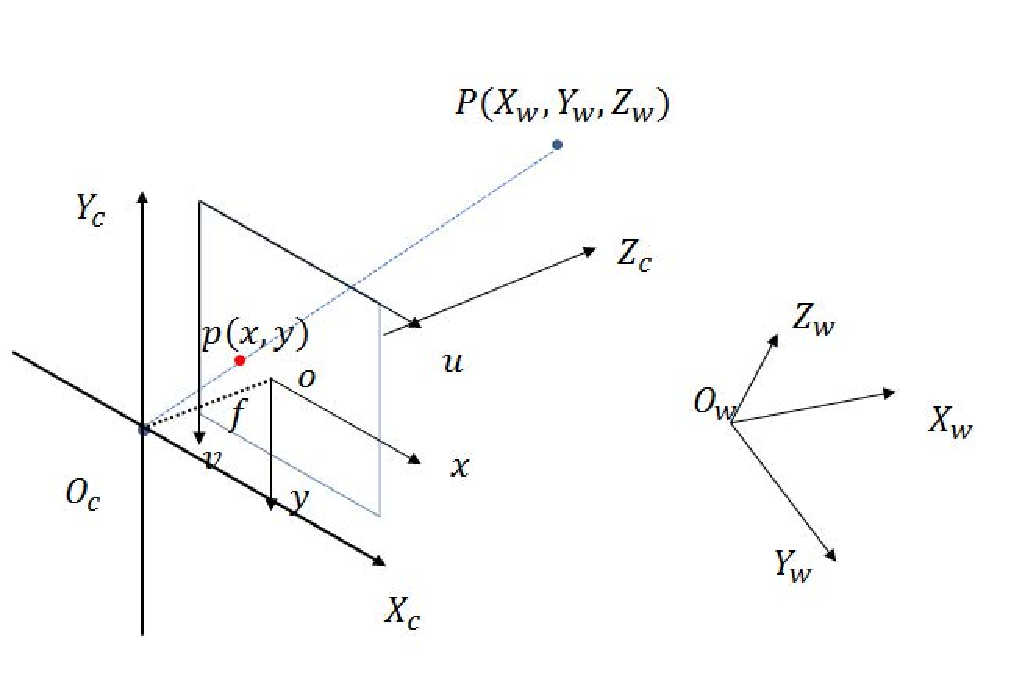
\includegraphics[keepaspectratio,width=0.8\textwidth]{images/3_Ersteverfahren/Kamera/cameramodel.pdf}
 \caption{Modell einer Lochkamera}
 \label{fig:cameramodel}
\end{figure} 

Die vier Koordinatensysteme im Modell sind wie folgt definiert:

\begin{itemize}
	\item 3D Weltkoordinatensystem $P(X_W,Y_W,Z_W)$ \\
	Punktkoordinaten werden durch homogene Koordinaten dargestellt: $\widetilde{X_w}\sim(X_W,Y_W,Z_W,1)^T$
	\item 3D Kamerakoordinatensystem $C(X_C,Y_C,Z_C)$\\
	Punktkoordinaten werden durch homogene Koordinaten dargestellt: $\widetilde{X_c}\sim(X_C,Y_C,Z_C,1)^T$
	\item 2D Bildabbildung Koordinatensystem $p(x,y)$\\
	Punktkoordinaten werden durch homogene Koordinaten dargestellt: $\widetilde{x}\sim(x,y,1)^T$
	\item 2D Bildpixel Koordinatensystem $I(u,v)$\\
	Punktkoordinaten werden durch homogene Koordinaten dargestellt: $\widetilde{u}\sim(u,v,1)^T$
\end{itemize}

% note
Unter diesem Modell wird ein 3D-Punkt im Weltkoordinatensystem durch drei Koordinaten den 2D-Bildpixelkoordinaten zugeordnet.

(\textbf{1}). 3D-Weltkoordinatensystem zum 3D-Kamera-Koordinatensystem.

Die Transformation vom Weltkoordinatensystem zum Kamerakoordinatensystem ist eine Starrekörpertransformation, d.h. das Objekt verformt sich nicht und nur durch Rotation und Parallelverschiebung. Diese Transformation wird in Abbildung \ref{fig:WzuC} gezeigt. R bedeutet Rotationsmatrix und T ist Translationsmatrix.

\begin{figure}[htb]
 \centering 
 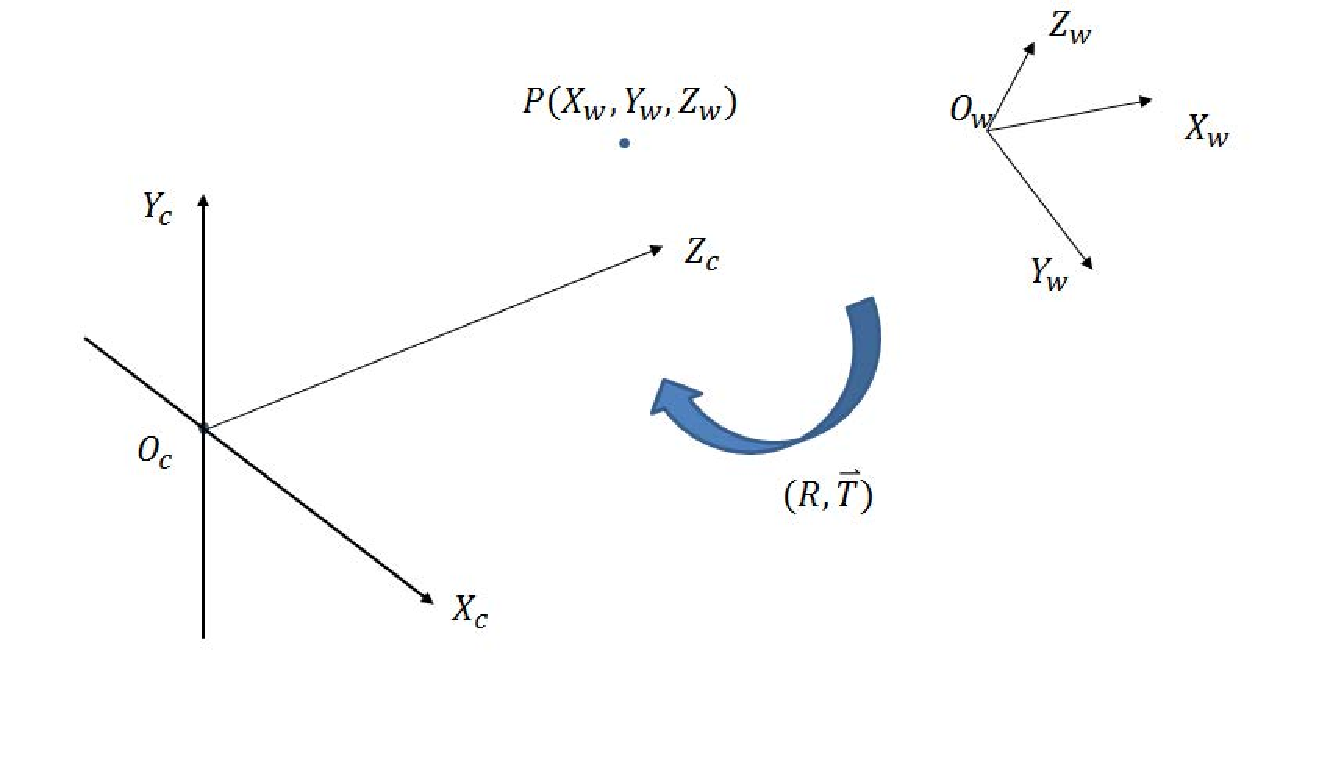
\includegraphics[keepaspectratio,width=0.8\textwidth]{images/3_Ersteverfahren/Kamera/WzuC.pdf}
 \caption{Transformation vom Weltkoordinatensystem zum Kamerakoordinatensystem}
 \label{fig:WzuC}
\end{figure} 

Um die entsprechende Rotationsmatrix zu erhalten, wird verschiedene Winkel um verschiedene Koordinatenachsen gedreht. Ein simple Beispiel wird in Abbildung \ref{fig:rotation} gezeigt.

\begin{figure}[H]
 \centering 
 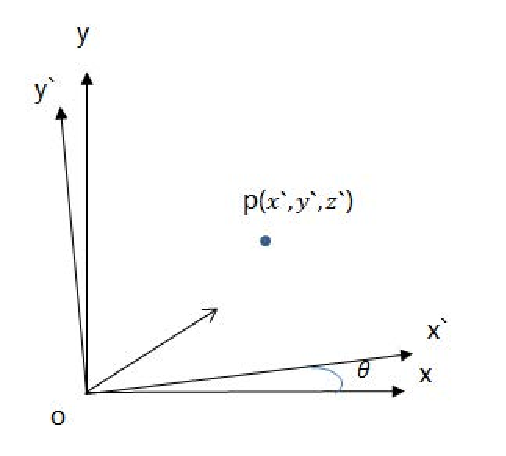
\includegraphics[keepaspectratio,width=0.4\textwidth]{images/3_Ersteverfahren/Kamera/rotationsmatrix.pdf}
 \caption{Rotation um Z-Achse}
 \label{fig:rotation}
\end{figure} 

Aus dem Bild können wir leicht bekommen:

\begin{equation}
   \begin{cases} 
	x = x'\cos\theta - y'\sin\theta \\	
	y = x'\sin\theta + y'\cos\theta \\
	z = z'
	\end{cases}
\end{equation}

In Matrixform wie folgend ausgedrückt:

\begin{equation}
   \begin{bmatrix}
	x \\  
	y \\
	z
	\end{bmatrix} = \begin{bmatrix}
	\cos\theta & -\sin\theta & 0	\\
	\sin\theta & \cos\theta  & 0	\\
	0    	   & 0           & 1	
	\end{bmatrix} \cdot \begin{bmatrix}
	x' \\  
	y' \\
	z'
	\end{bmatrix}= R_1 \cdot \begin{bmatrix}
	x' \\  
	y' \\
	z'
	\end{bmatrix}
\end{equation}

In ähnlicher Weise, um die x-Achse, y-Achse dreht sich um $\varphi$ und $\omega$ Grad, bekommen:
\begin{equation}
   \begin{bmatrix}
	x \\  
	y \\
	z
	\end{bmatrix} = \begin{bmatrix}
		1   & 0          & 0	\\
		0   & \cos\varphi & -\sin\varphi	\\
	    0   & \sin\varphi& \cos\varphi	
	\end{bmatrix} \cdot \begin{bmatrix}
	x' \\  
	y' \\
	z'
	\end{bmatrix}= R_2 \cdot \begin{bmatrix}
	x' \\  
	y' \\
	z'
	\end{bmatrix}
\end{equation}

\begin{equation}
   \begin{bmatrix}
	x \\  
	y \\
	z
	\end{bmatrix} = \begin{bmatrix}
	\cos\omega  & 0           & \sin\omega	\\		
	0    	    & 1           & 0	\\
	-\sin\omega &0            &  \cos\omega
	\end{bmatrix} \cdot \begin{bmatrix}
	x' \\  
	y' \\
	z'
	\end{bmatrix}= R_3 \cdot \begin{bmatrix}
	x' \\  
	y' \\
	z'
	\end{bmatrix}
\end{equation}

Dann können die Rotationsmatrix erhalten werden:
\begin{equation}
   R = R_1 \cdot R_2 \cdot R_3
\end{equation}

Kombinieren das Obige, können die Koordinaten von Punkt P im Kamerakoordinatensystem erhalten.
\begin{equation}
   \begin{bmatrix}
	X_C \\  
	Y_c \\
	Z_c
	\end{bmatrix} = R \cdot \begin{bmatrix}
	X_w \\  
	Y_w \\
	Z_w 
	\end{bmatrix} +T
\end{equation}

Im homogenen Koordinatensystem darstellt:
\begin{equation}
   \begin{bmatrix}
	X_C \\  
	Y_C \\
	Z_C \\
	1
	\end{bmatrix} = \begin{bmatrix}
	R & t	\\
	\vec{0}	& 1 \\
	\end{bmatrix} \cdot \begin{bmatrix}
	X_w \\  
	Y_w \\
	Z_w \\
	1
	\end{bmatrix}
\end{equation}

(\textbf{2}). 3D-Kamera-Koordinatensystem zum 2D-Bildabbildung Koordinatensystem.

Die Transformation vom Kamerakoordinatensystem zum Bildkoordinatensystem gehört zur perspektivischen Projektionsbeziehung von 3D zu 2D, wie zeigt in Abbildung \ref{fig:Czuimage}.

\begin{figure}[H]
 \centering 
 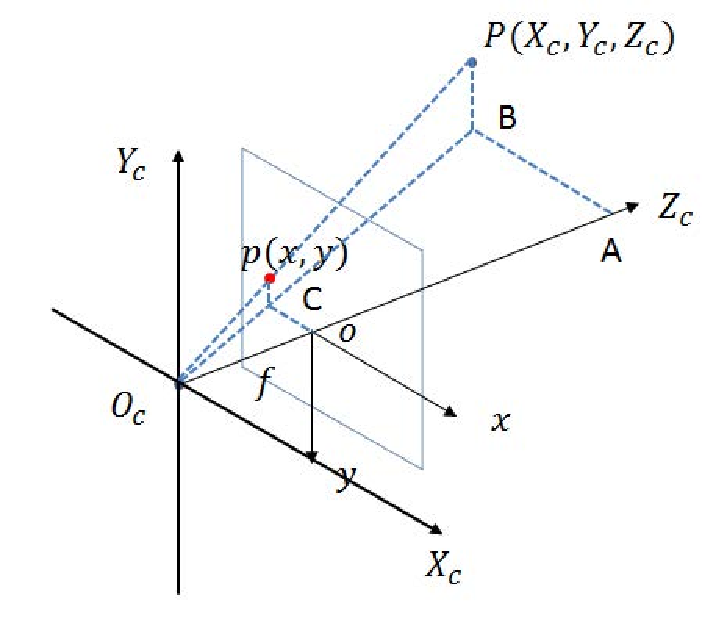
\includegraphics[keepaspectratio,width=0.4\textwidth]{images/3_Ersteverfahren/Kamera/Czuimage.pdf}
 \caption{Transformation vom Kamerakoordinatensystem zum Bild Koordinatensystem}
 \label{fig:Czuimage}
\end{figure} 

Es gibt zwei Paare ähnlichen Dreiecken:
\begin{equation}
   \begin{split}
    \triangle ABO_C \sim \triangle oCO_c\\  
	\triangle PBO_C \sim \triangle pCO_c
	\end{split}
\end{equation}

Aus ähnlichen Dreiecksbeziehungen können diese Gleichung Verfügbar sein:
\begin{equation}
   \frac{AB}{oC} = \frac{AO_C}{oO_C} = \frac{PB}{pC} = \frac{X_C}{x} = \frac{Z_C}{f} = \frac{Y_C}{y} 
\end{equation}

Durch die Gleichung Transformation können es erhalten: 
\begin{equation}
   x = f \cdot \frac{X_C}{Z_C}, y = f \cdot \frac{Y_C}{Z_C}
\end{equation}

Im homogenen Koordinatensystem darstellt:
\begin{equation}
   Z_C \cdot \begin{bmatrix}
	x \\  
	y \\
	1
	\end{bmatrix} = \begin{bmatrix}
	f & 0 & 0 & 0	\\
	0 & f & 0 & 0	\\
	0 & 0 & 1 & 0	
	\end{bmatrix} \cdot \begin{bmatrix}
	X_C \\  
	Y_C \\
	Z_C \\
	1
	\end{bmatrix}
\end{equation}

Zu dieser Zeit ist die Einheit des Projektionspunkts p noch nicht Pixel, sondern mm und muss weiter in das Pixelkoordinatensystem umgewandelt werden.

(\textbf{3}). 2D-Bildabbildung Koordinatensystem zum 2D-Bildpixel Koordinatensystem.

Das Pixelkoordinatensystem und das Bildkoordinatensystem befinden sich alle auf der Abbildungsebene, aber die jeweiligen Ursprünge und Maßeinheiten sind unterschiedlich. Der Ursprung des Bildkoordinatensystems ist der Schnittpunkt der optischen Achse der Kamera und der Abbildungsebene, üblicherweise der Mittelpunkt der Abbildungsebene oder der Hauptpunkt. Die Einheit des Bildkoordinatensystems ist mm, die zu der physikalischen Einheit gehört, und die Einheit des Pixelkoordinatensystems ist Pixel. Wir beschreiben gewöhnlich, dass ein Pixel welche Zeilen und Spalten ist. So ist der Übergang zwischen den beiden wie folgt in Abbildung \ref{fig:Konvertierung von Pixelkoordinatensystem zu Bildkoordinatensystem}. 

\begin{figure}[H]
 \centering 
 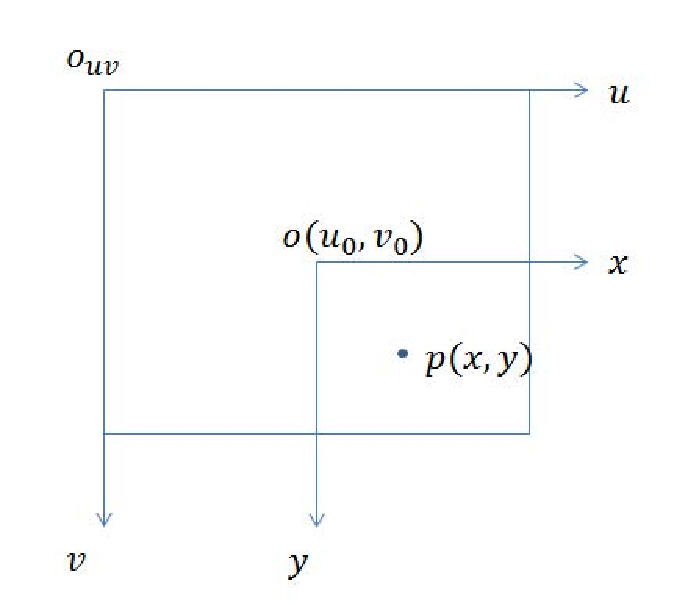
\includegraphics[keepaspectratio,width=0.5\textwidth]{images/3_Ersteverfahren/Kamera/imagezupixel.pdf}
 \caption{Konvertierung von Bildkoordinatensystem zu Pixelkoordinatensystem}
 \label{fig:Konvertierung von Pixelkoordinatensystem zu Bildkoordinatensystem}
\end{figure} 

Hier dx, dy ist die Größe jedes Pixels in den X- und Y-Achsenrichtungen. Jedes Pixel des Bildes hat die folgende Beziehung zwischen den zwei Koordinatensystemen.

\begin{equation}
   \begin{cases} 
	u = \frac{x}{d_x} + u_0	 \\  
	v = \frac{y}{d_y} + v_0	
	\end{cases}
\end{equation}

Im homogenen Koordinatensystem darstellt:

\begin{equation}
   \begin{bmatrix}
	u \\  
	v \\
	1
	\end{bmatrix} = \begin{bmatrix}
	\frac{1}{d_x} 			& 0 			& u_0	\\
	0	 					& \frac{1}{d_y} & v_0	\\
	0     					& 0 			& 1	
	\end{bmatrix} \cdot \begin{bmatrix}
	x \\  
	y \\
	1
	\end{bmatrix}
\end{equation}

Es ist erwähnenswert, dass Bildkoordinatensystem ist eine zweidimensionale Ebene(Bildebene), in praktisch die Oberfläche des Kamera-CCD-Sensors ist. Jeder CCD-Sensor hat eine bestimmte Größe und eine bestimmte Auflösung. Diese beide bestimmt die Konvertierungsbeziehung. Geben eine simple Beispiel, eine Größe des CCD-Sensors ist $\SI{8}{\mm} \times \SI{6}{\mm}$ , die Auflösung dafür ist $640~pixels \times 480~pixels$, dann die Beziehung zwischen mm und Pixel läuft $80~pixel/mm$. Lassen Sie die physikalische Größe jedes Pixels des CCD-Sensors $d_x \times d_y$ sein, entspricht läuft $d_x = d_y = \SI{1/80}{\mm}$.
 
Dann durch die Umwandlung der obigen vier Koordinatensysteme kann ein Punkt vom Weltkoordinatensystem zum Pixelkoordinatensystem erhalten.
\begin{equation}
\begin{split}
   Z_C \cdot \begin{bmatrix}
	u \\  
	v \\
	1
	\end{bmatrix} & = \begin{bmatrix}
	\frac{1}{d_x} 			& 0 			& u_0	\\
	0	 					& \frac{1}{d_y} & v_0	\\
	0     					& 0 			& 1	
	\end{bmatrix} \cdot \begin{bmatrix}
	f & 0 & 0 & 0	\\
	0 & f & 0 & 0	\\
	0 & 0 & 1 & 0	
	\end{bmatrix} \cdot \begin{bmatrix}
	R & t	\\
	\vec{0}	& 1 \\
	\end{bmatrix} \cdot \begin{bmatrix}
	X_w \\  
	Y_w \\
	Z_w \\
	1
	\end{bmatrix} \\
	& = \begin{bmatrix}
	f_x & 0 & u_0 & 0	\\
	0 & f_y & v_0 & 0	\\
	0 & 0 & 1 & 0	
	\end{bmatrix} \cdot \begin{bmatrix}
	R & t	\\
	\vec{0}	& 1 \\
	\end{bmatrix} \cdot \begin{bmatrix}
	X_w \\  
	Y_w \\
	Z_w \\
	1
	\end{bmatrix}
\end{split}	
\end{equation}

Die erste Matrix der rechten Gleichung ist die allgemein bekannt interne Referenz der Kamera. Dagegen ist die zweite Matrix die externe Referenz der Kamera. Beide Parameter der Kamera durch Zhang Zhengyou \cite{zhangzhengyou} Kalibrierung erhalten werden. Einige typisch Kamera Parameter von Manufaktur liegt in Tabellen \ref{tbl:params}.

\begin{table}[htb]
	\captionabove{Parameter des Kameras im Vergleich}
	\label{tbl:params}
	\footnotesize
	\centering
	\rowcolors{2}{white}{gray!25}	%TUgreen!25
	\begin{tabular}{|p{3cm}|p{2.5cm}|p{2.5cm}|p{2.5cm}|}	%p{}m{}b{}clr
	\toprule
	\textbf{Parameter} & \textbf{Google Pixel} & \textbf{Google Pixel2} & \textbf{Iphone 10}\\
	\midrule
	Sensor Größe $''$ & 1/2.3 & 1/2.6 & 1/3 \\
	Bild Auflösung $pixels$ & $4048 \times 3036$ & $4032 \times 3024$ & $4032 \times 3024$ \\
	Pixel Größe $\mu m$ & 1.544 & 1.4 & 1.22 \\	
	Brennweite $mm$ & 4.67 & 4.47 & 3.99 \\
	Formatfaktor $35 mm$  	&5.55	&6.04	&7.02	\\
	
	\bottomrule
	\end{tabular}
\end{table} 



Aus der obigen Formel wenn die internen und externen Parameter der Kamera bekannt sind, ist nämlich die Projektionsmatrix bekannt, und zu diesem Zeitpunkt können die entsprechenden Bildkoordinaten für jeden beliebigen räumlichen Punkt erhalten werden. Dagegen  wenn die Position $m(u,v)$ in Bildkoordinate bekannt ist, und auch die Parameter innerhalb und außerhalb der Kamera bereits bekannt sind, kann die entsprechenden Punkt in Wert Koordinate nicht eindeutig bestimmt werden. Die Grund dafür ist, die $Z_c$ Information während des Projektionsprozesses eliminiert wird. 

\textbf{Umwandelung  Modelle}

Als nächstes machen die Umwandlungsbeziehung zwischen den entsprechenden Punkten in den beiden Bilder.
Zuerst wird in diese Arbeit eine vereinfachte Situation  betrachten, d.h. nur mit Rotations Einfluss. Abbildung \ref{fig:rotationsmodel} zeigt das 3D-Rotationsbewegungsmodell der Kamera. Darin die Position des optischen Zentrums ändert sich während der Kamerabewegung im Drehbewegungsmodell der Kamera nicht. Unter diesem Modell ist die Abbildungsbeziehung zwischen dem Punkt X im Weltkoordinatensystem und der Bildkoordinate x im homogenen Koordinatensystem dargestellt: 
\begin{equation}
   x = KRX, X = \lambda  K^{-1} x
\end{equation}

Wobei: K ist der interne Parameter der Kamera, wie zuvor definiert. $\lambda$ ist der unbekannte Skalierungsfaktor, d.h. unter dem Kameramodell die Quelle der Bildpunktkoordinaten einem Strahl zugeordnet ist.

\begin{figure}[H]
 \centering 
 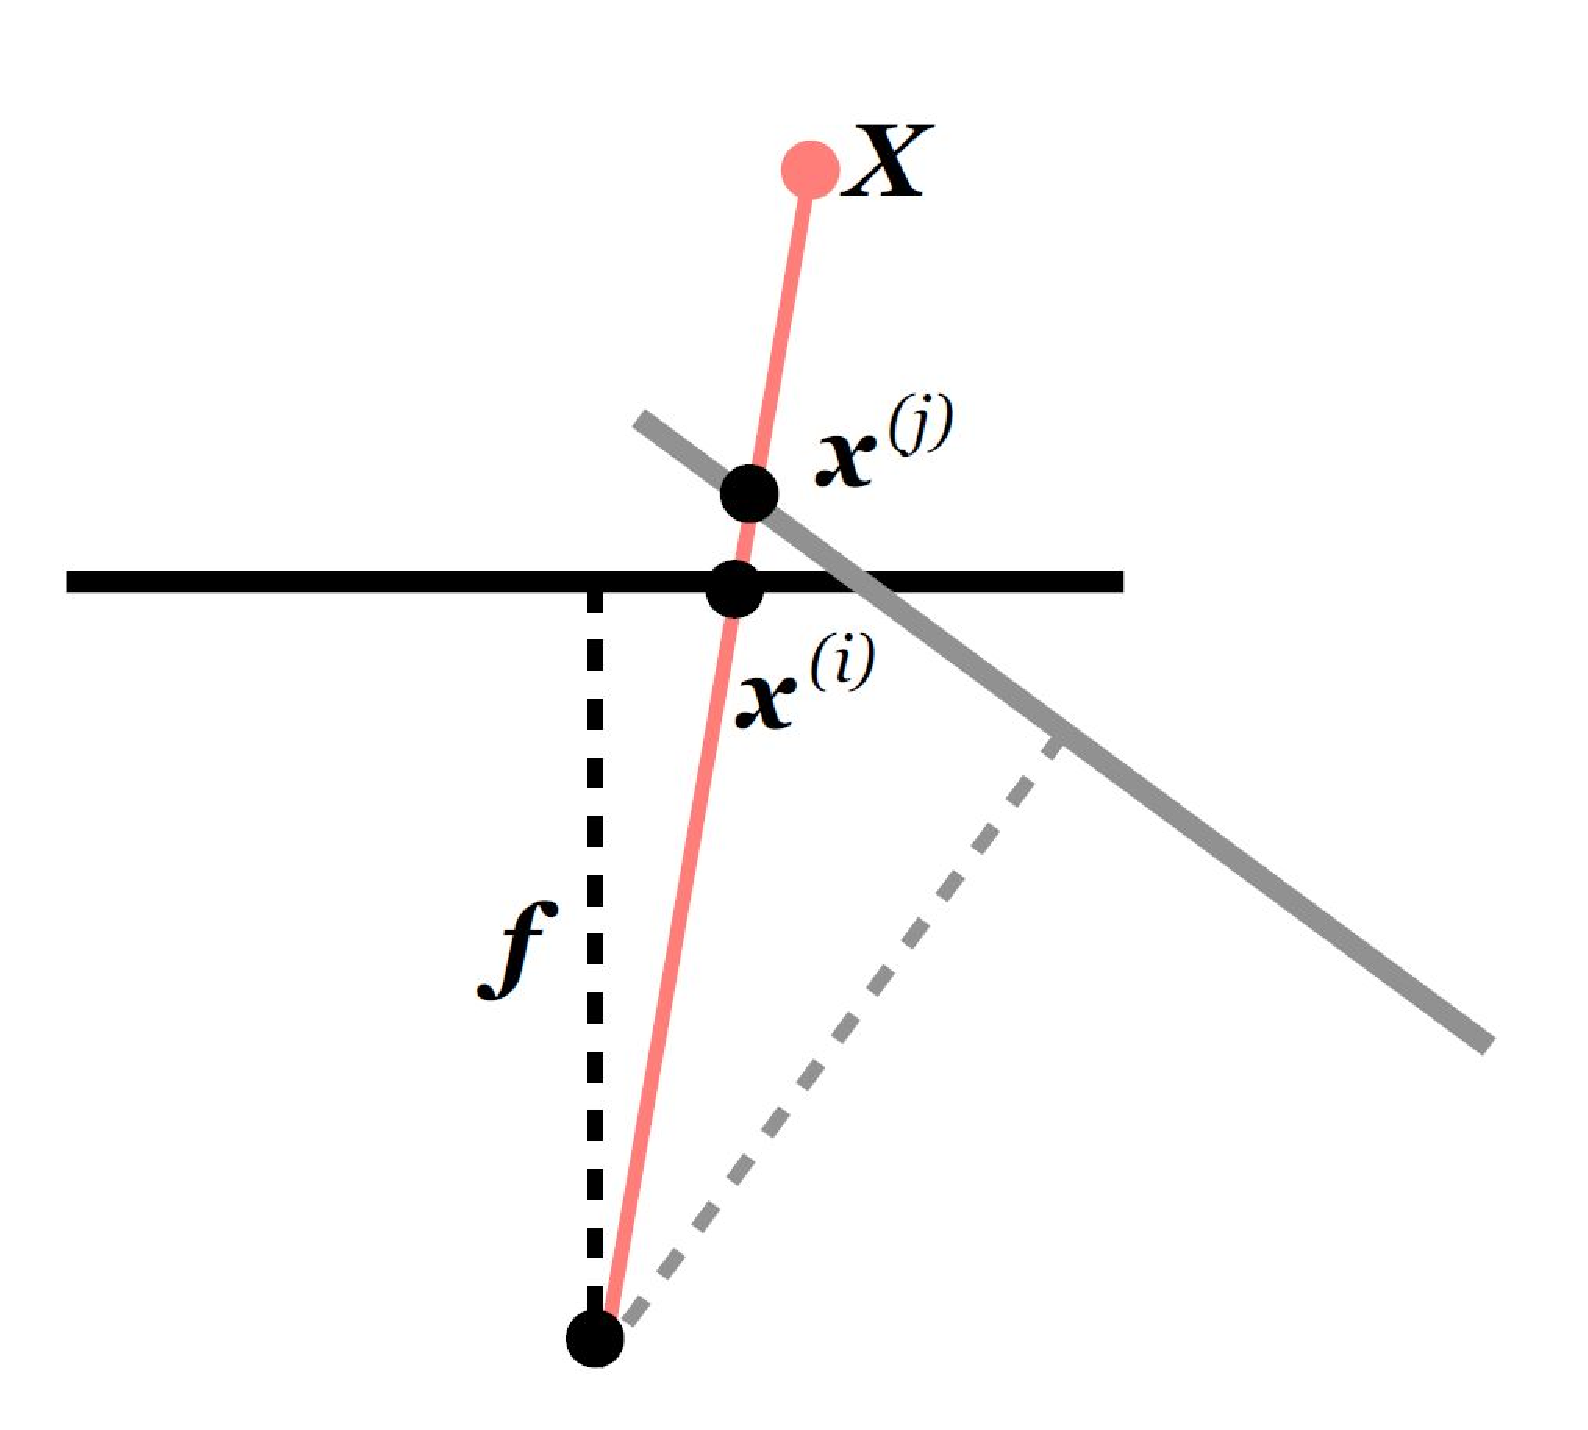
\includegraphics[keepaspectratio,width=0.5\textwidth]{images/3_Ersteverfahren/Kamera/rotationsmodel.pdf}
 \caption{Rotationsbewegungsmodell}
 \label{fig:rotationsmodel}
\end{figure} 


Herleiten nun die Beziehung zwischen Bildpunkten in einem Framepaar für zwei verschiedene Kameraausrichtungen (siehe Abbildung \ref{fig:rotationsmodel}). Für einen Weltkoordinatepunkt X sind die projizierten Punkte $x_i$ und $x_j$ in der Bildebene von zwei Bildern i und j gegeben durch
\begin{equation}
   x_i = KR_iX, x_j = KR_jX
\end{equation}

Anordnen diese Gleichungen weiter und ersetzen X, wird eine Beziehung aller Punkte im Bildrahmen i auf alle Punkte im Rahmen j erhalten:
\begin{equation}
   x_j = KR_jR_i^TK^{-1}x_i
\end{equation}

Bisher wird nur die Beziehung zwischen zwei Bildern desselben Videos betrachtet. Lockern diese Einschränkung, indem Frames von einer Kamera, die sich gemäß $R$ dreht, zu einer anderen Kamera, die sich gemäß $R'$ dreht, abbilden. Es gibt eine Hypothese, dass beide Kamerazentren sich im Ursprung befinden. Dann die Warping-Matrix, die Punkte von einer Kamera auf die andere abbildet, definiert werden können:
\begin{equation}
   W = KR'R^TK^{-1}
\end{equation}

Es wird hier angenommen, dass das erste Bild als Referenz Bild nehmen und der Rotationswinkel 0 ist. Dann die Gleichung kann vereinfacht als:
\begin{equation}
   W = KRK^{-1}
\end{equation}

Kombiniert mit Formel 4.23 können es ausgedrückt als:
\begin{equation}
   x_j = Wx_i
\end{equation}

Diese Formel zeigt, dass jeder Punkt in dem Bild i nach der Transformationsmatrix W in einen entsprechenden Punkt in dem Bild j umgewandelt werden kann. Weiter in einem allgemeineren Fall, d.h. derzeit nicht nur mit Rotations Einfluss, sondern auch Translations Einfluss nehmen. Das Ableitungsverlauf ist im Allgemeinen gleich. Der Hauptunterschied ist Anzahl der Parametern, die von original nur 3 Rotationsparameter zur jetzt 6 Parameter einschließlich 3 Rotationsparameter und 3 Translationsparameter. Das neu Warping-Matrix darstellt wie folgen:

\begin{equation}
   W = \begin{bmatrix}
	f			& 0 		& \frac{w}{2}	  & 0 \\
	0	 		& f			& \frac{h}{2} 	  & 0 \\
	0     		& 0 		& 1 			  & 0 \\	
	0     		& 0 		& 0 			  & 1
	\end{bmatrix} \cdot \begin{bmatrix}
	R_{11}			& R_{21}  		& R_{31}	  & 0 \\
	R_{12}	 		& R_{22}		& R_{32}	  & 0 \\
	R_{13}     		& R_{23} 		& R_{33} 	  & 0 \\	
	t1     			& t2 			& t3 		  & 1
	\end{bmatrix} \cdot \begin{bmatrix}
	\frac{1}{f}	   & 0 				& -\frac{w}{2f}	  & 0 \\
	0	 		   & \frac{1}{f}	& -\frac{h}{2f}   & 0 \\
	0     		   & 0 		        & 1 			  & 0 \\	
	0     		   & 0 		        & 0 			  & 1
	\end{bmatrix}
\end{equation}

\textbf{Transformation Optimierung}

In den letzten beiden Abschnitten wurde die Transformationsmatrix zwischen den beiden Bilder aus dem Kameramodell abgeleitet. Hier in diesen Abschnitt werden die Parameter der Transformationsmatrix berechnet, also bestimmen das Transformationsmatrix. Hier sind die entsprechenden Punkte von zwei benachbarten Bildern $x_i, x_j$ bekannt, und die Umwandlungsbeziehung dazwischen wird als die Formel 4.26 gezeigt. Angesichts dieser Bedingung 
kann die Berechnung des Transformationsmatrix als ein Optimierungsproblem formulieren, wobei den Fehler J bei der Mittelwertbildung im Quadrat aller Punktkorrespondenzen minimieren wollen:

\begin{equation}
   J = \sum_{(i,j)}\lVert x_j - Wx_i \rVert ^2
\end{equation}

Beachten, dass dies ein nichtlineares Optimierungsproblem ist. Einige nichtlinearer Optimierer könnte verwendet werden, um diese Zielfunktion zu minimieren. Jedoch ist es gefunden, dass Koordinatenabstieg durch direkte objektive Funktionsbewertung schnell konvergiert. Jedes Mal, wenn einen Schritt gemacht wird, bei dem die Zielfunktion J nicht abnimmt, kehren die Schrittrichtung um und verringern die Schrittweite des entsprechenden Parameter. Der Algorithmus endet, sobald die Schrittgröße für alle Parameter unter einen gewünschten Schwellenwert fällt (d.h. Wenn eine Zielgenauigkeit erreicht haben). 

Der detaillierte Algorithmus ist wie folgt darstellt. Einige Definitionen werden hier einführen. $P_0$ heißt der Vektor, die Anfangswerte der Parameter speichert. Anschießen in den Vektor $d_p$ speichert die Schrittgröße jedes Parameters. $temp_dp$ ist der Vektor, in den die gewünschten Schwellenwert der Parameter speichert. D bedeutet die Anzahl der Unbekannter Parameter und W das Transformationsmatrix.

1. Zuerst durch Anfangswert $P_0$ berechnen den anfänglich Fehler $J_0$.

2. Verändern einen Parameter in einer entsprechenden Schrittrichtung mit entsprechenden Schrittgröße.

3. Berechnen den neuen Fehler $J_new$.

4. Vergleichen die beiden Fehler, ob der neu Fehler $J_new$ kleiner ist. Wenn Ja bestimmt, behalten diesen Wert und ändern des Objekt auf den nächsten Parameter. Kehren zum zweiten Schritt zurück. Dagegen kehren die Schrittrichtung um und verringern die Schrittgröße des Parameter auf ein Drittel des Originals. Ändern des Objekt auf den nächsten Parameter und kehren zum zweiten Schritt zurück.

5. Wenn alles Schrittgröße in $d_p$ die zuvor festgelegter Schwellenwert erreicht, beenden das Algorithmus und geben den minimalen Fehler J und entsprechenden Transformationsmatrix aus.

Das Flussdiagramm des Algorithmus ist wie in Abbildung \ref{fig:FlussdiagrammforOptimierung} darstellt.

Dann durch Transformationsmatrix können die Koordinaten des zweiten Bildes in die Koordinaten des ersten Bildes umgewandelt werden. Abbildung \ref{fig:Transformation in eine Koordinate} zeigt diese Verlauf. Dann durch Subtraktion können die Differenzbild erhalten.

\begin{figure}[H]
 \centering 
 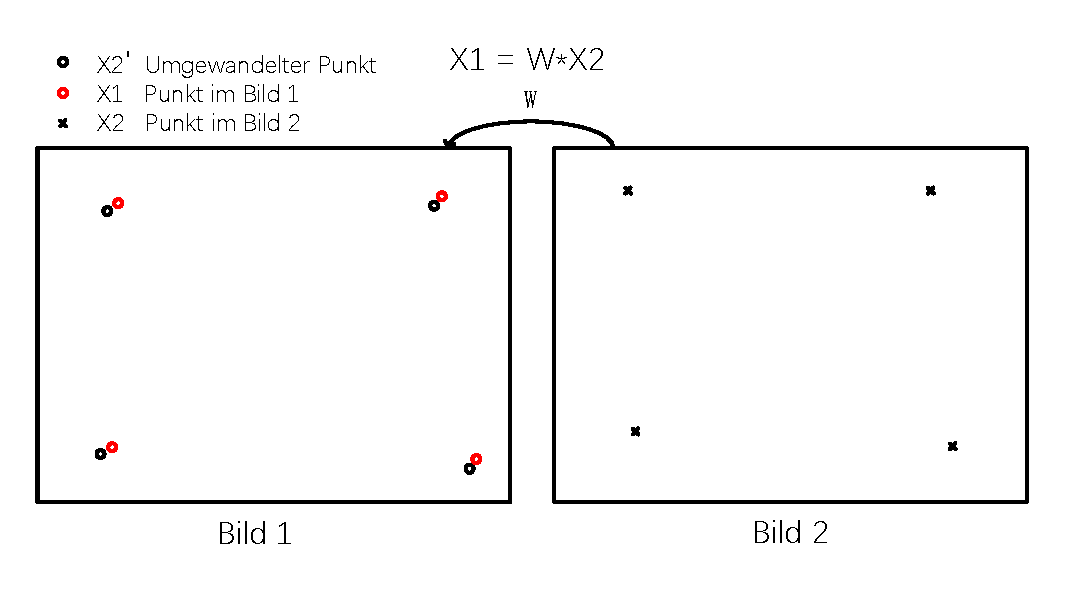
\includegraphics[keepaspectratio,width=0.8\textwidth]{images/3_Ersteverfahren/Kamera/Transformmatrix.pdf}
 \caption{Transformation in desselben Koordinate}
 \label{fig:Transformation in eine Koordinate}
\end{figure} 

\begin{figure}[H]
 \centering 
 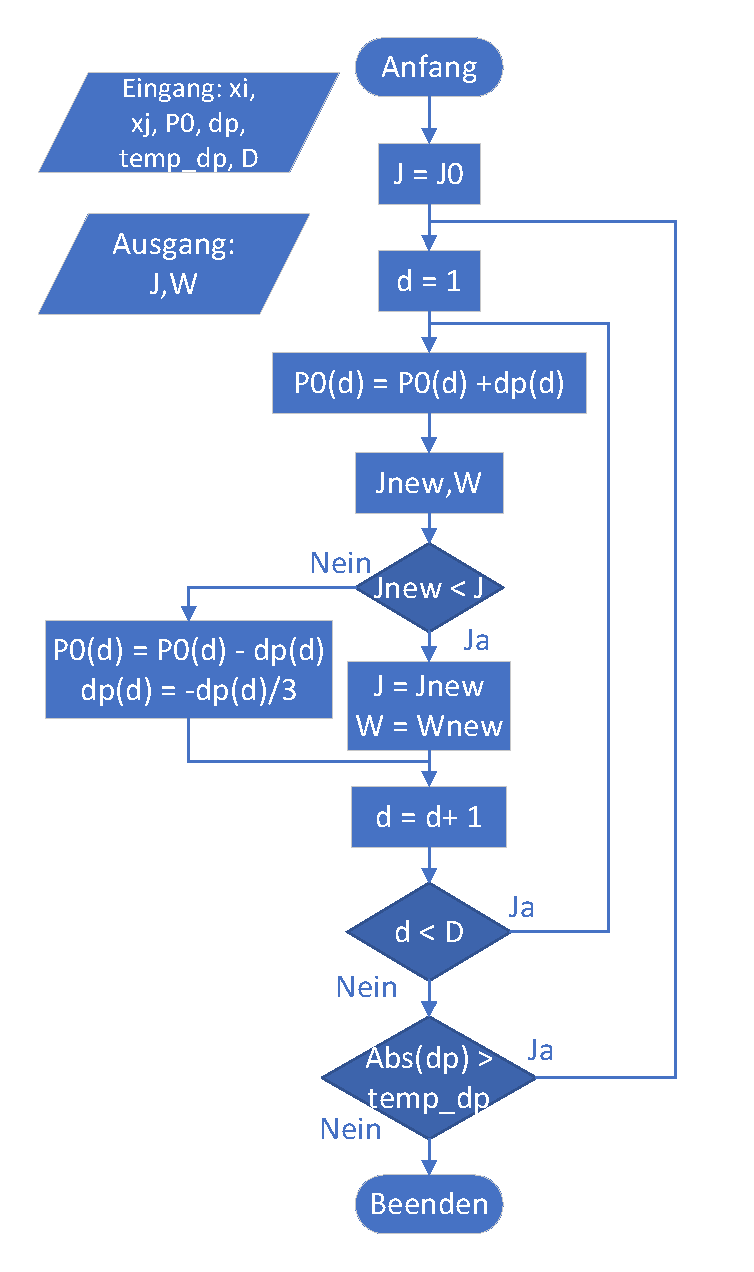
\includegraphics[keepaspectratio,width=0.8\textwidth]{images/3_Ersteverfahren/Kamera/flussdiagramm_for_parameter.pdf}
 \caption{Flussdiagramm für Optimierung}
 \label{fig:FlussdiagrammforOptimierung}
\end{figure} 



\section{Differenzbild Optimierung}
Durch Bildregistration erhalten eine Reihe Bilder von der Kamera, deren Koordinaten in dasselbe Koordinatensystem umgewandelt wurden. Auswälen je zwei Bilder und subtrahieren, um eine Reihe Differenzbildern zu enthälten. Die Ziel in diesem Abschnitt ist von diese Differenzbildern ein detektierendes Bilder herstellen, dadurch die QR Muster Detektion vereinfachen werden können. Es sollte hier beachtet werden, dass aufgrund der Zeitsynchronisation die QR Muster in Differenzbilder einige unerwartete Situation aufgetreten sein können. Einige mögliche Formel der Differenzbilder wie folgend gezeigt. Nehmen an, dass es in der vertikalen Richtung ist.

\begin{itemize}
	\item total Schwarz-Weiß-Schwarz-Weiß-Schwarz Ordnung.
	\item halb Schwarz-Weiß-Schwarz-Weiß-Schwarz Ordnung, halb nicht gezeigt.
	\item total Weiß-Schwarz-Weiß-Schwarz-Weiß Ordnung.
	\item halb Weiß-Schwarz-Weiß-Schwarz-Weiß Ordnung, halb nicht gezeigt.
	\item halb Schwarz-Weiß-Schwarz-Weiß-Schwarz Ordnung, halb Weiß-Schwarz-Weiß-Schwarz-Weiß Ordnung.
	\item total nicht gezeigt.
\end{itemize}

Tabelle \ref{tbl:differenzbildformel} zeigt solche Situation und aufgelistet, ob sie zu folgend Detektion angepasst sind.

\begin{table}[htb]
	\captionabove{Die mögliche Differenzbilder}
	\label{tbl:differenzbildformel}
	\footnotesize
	\centering
	\rowcolors{2}{white}{gray!25}	%TUgreen!25
	\begin{tabular}{|p{2cm}<{\centering}|c|p{2cm}<{\centering}|c|}	%p{}m{}b{}clr p{3cm} p{8cm}
	\toprule
	\textbf{Ob angepasst zu folgende Detektion?} & \multirow{4}{*}{\textbf{Differenzbild}} & \textbf{Ob angepasst zu folgende Detektion?} & \multirow{4}{*}{\textbf{Differenzbild}} \\
	\midrule
	 Ja & 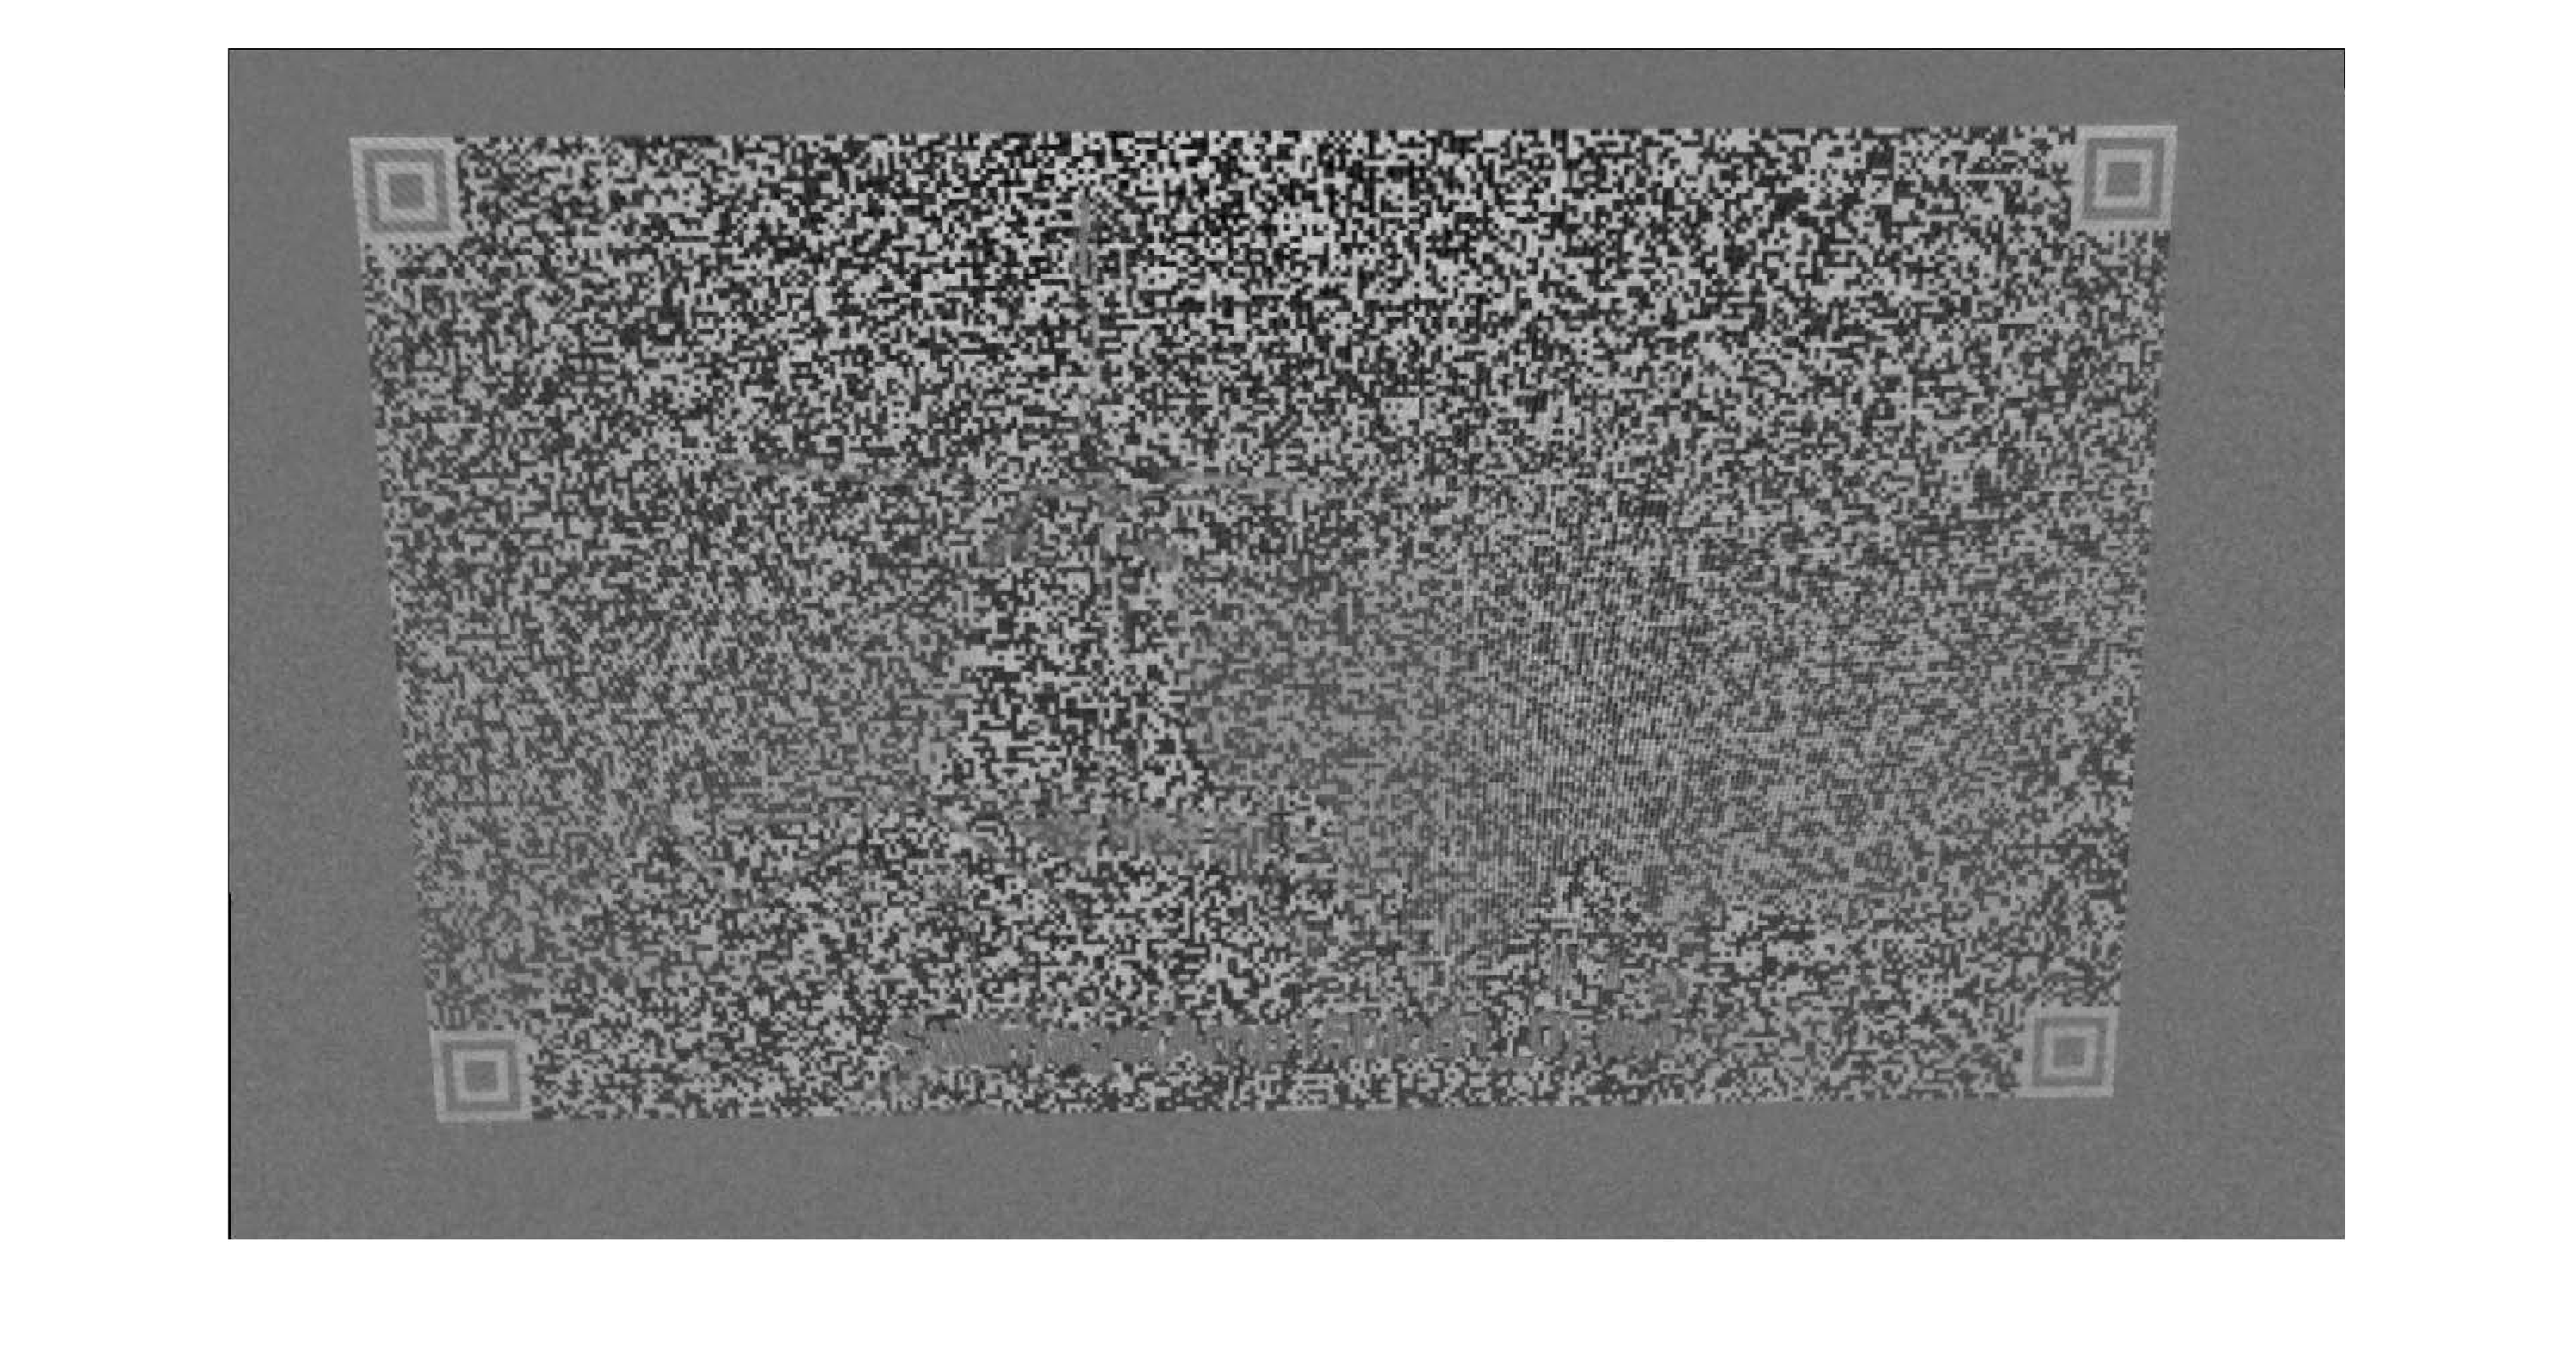
\includegraphics[scale=0.12]{images/3_Ersteverfahren/Differenzbild/0schwarz.pdf}& Nein & 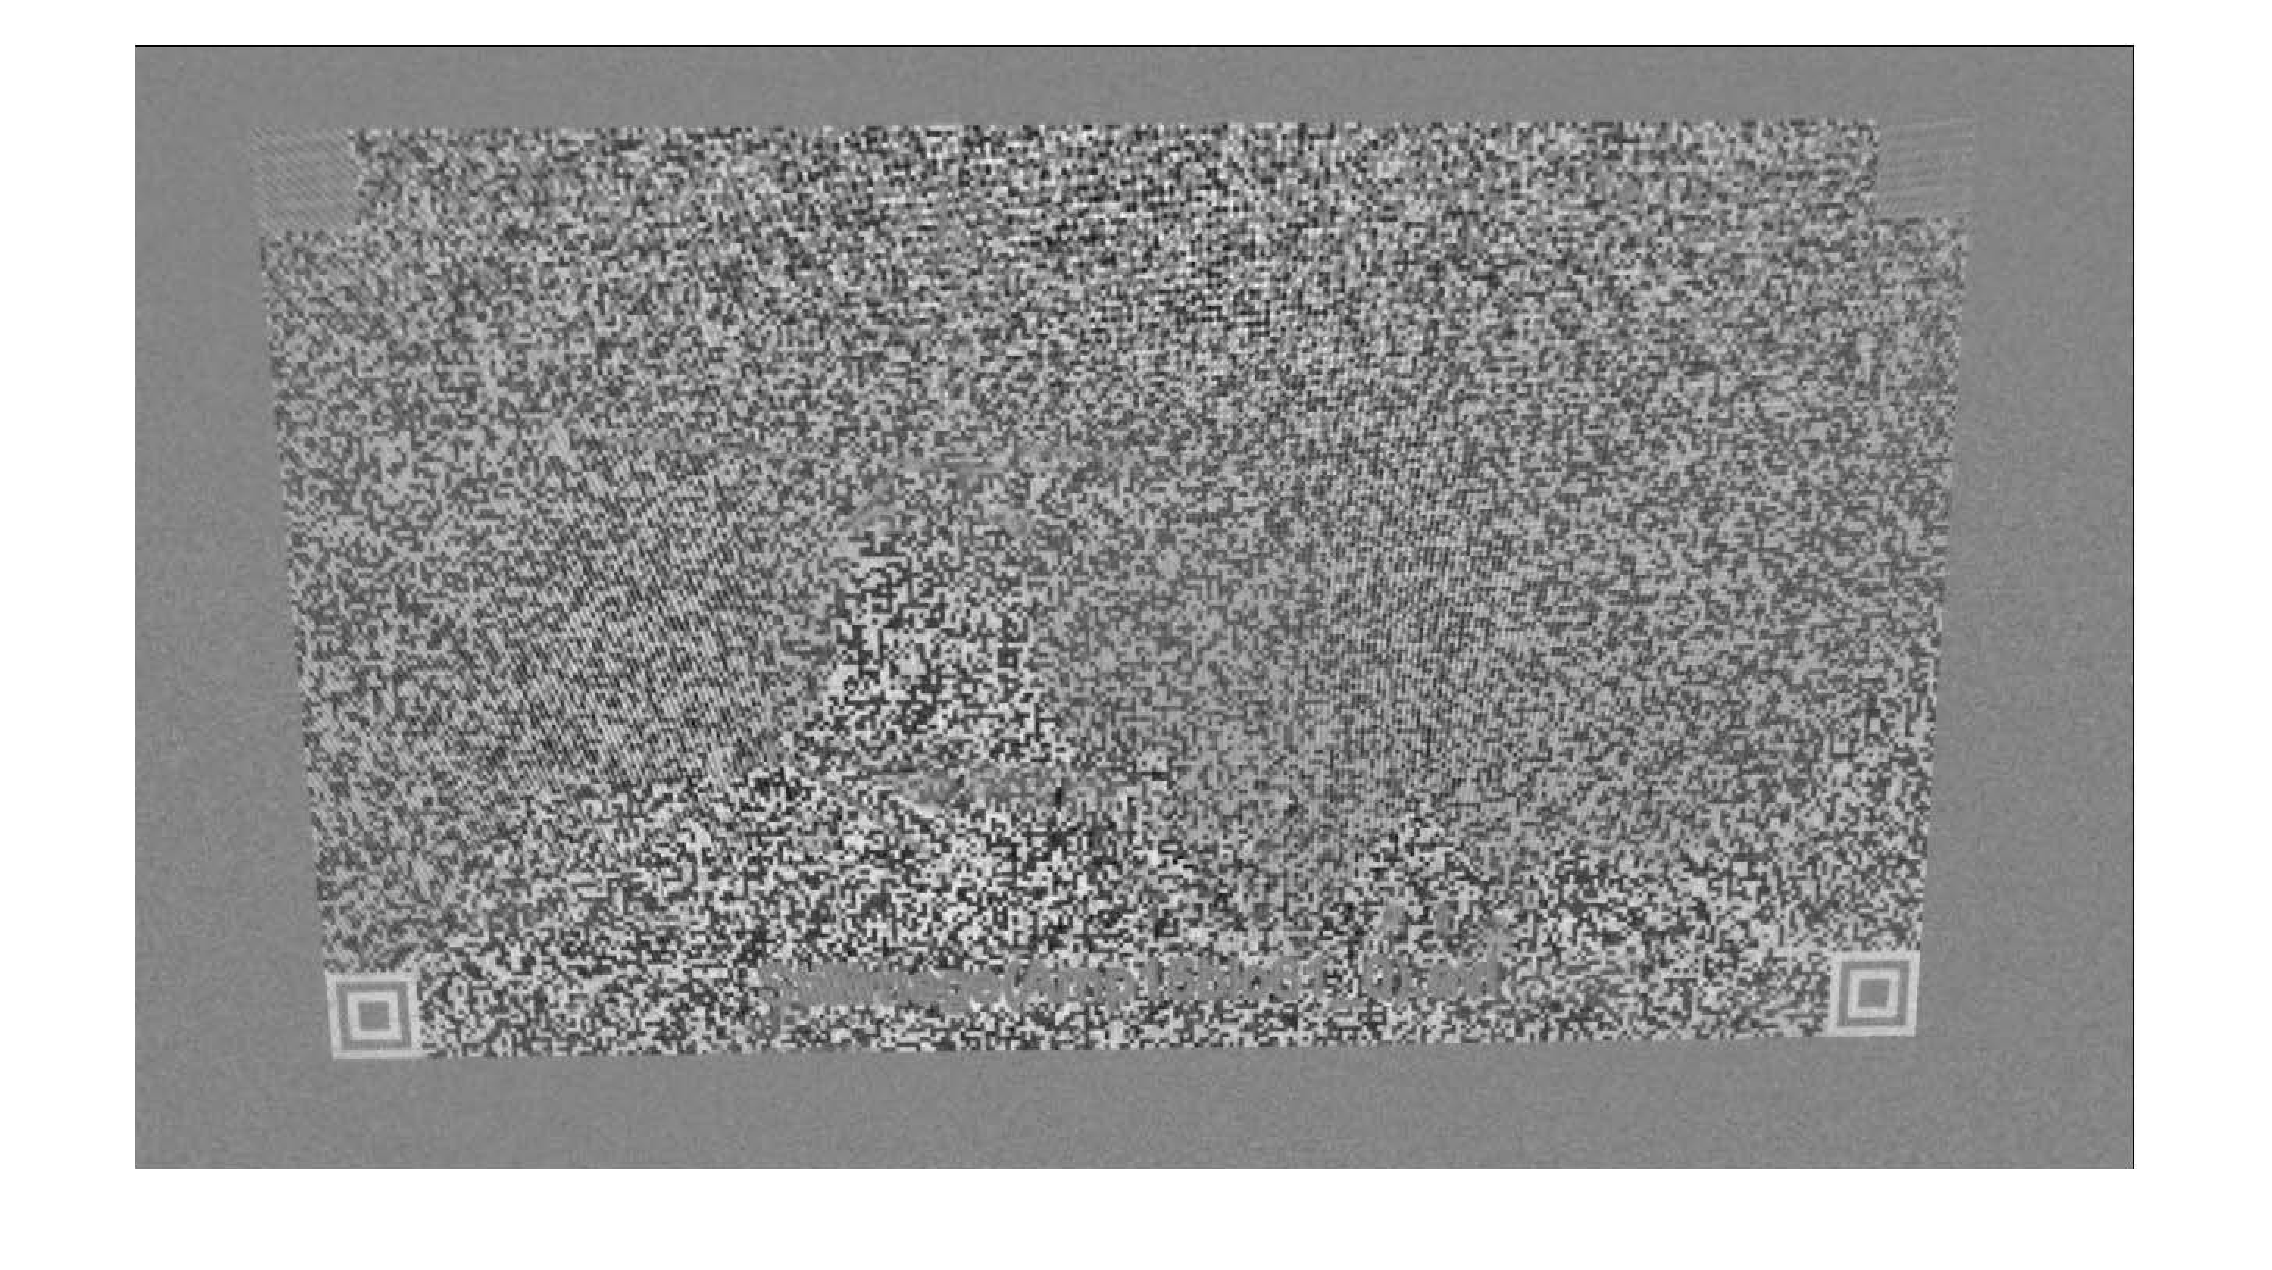
\includegraphics[scale=0.15]{images/3_Ersteverfahren/Differenzbild/1halfschwarz.pdf}\\
	Nein & 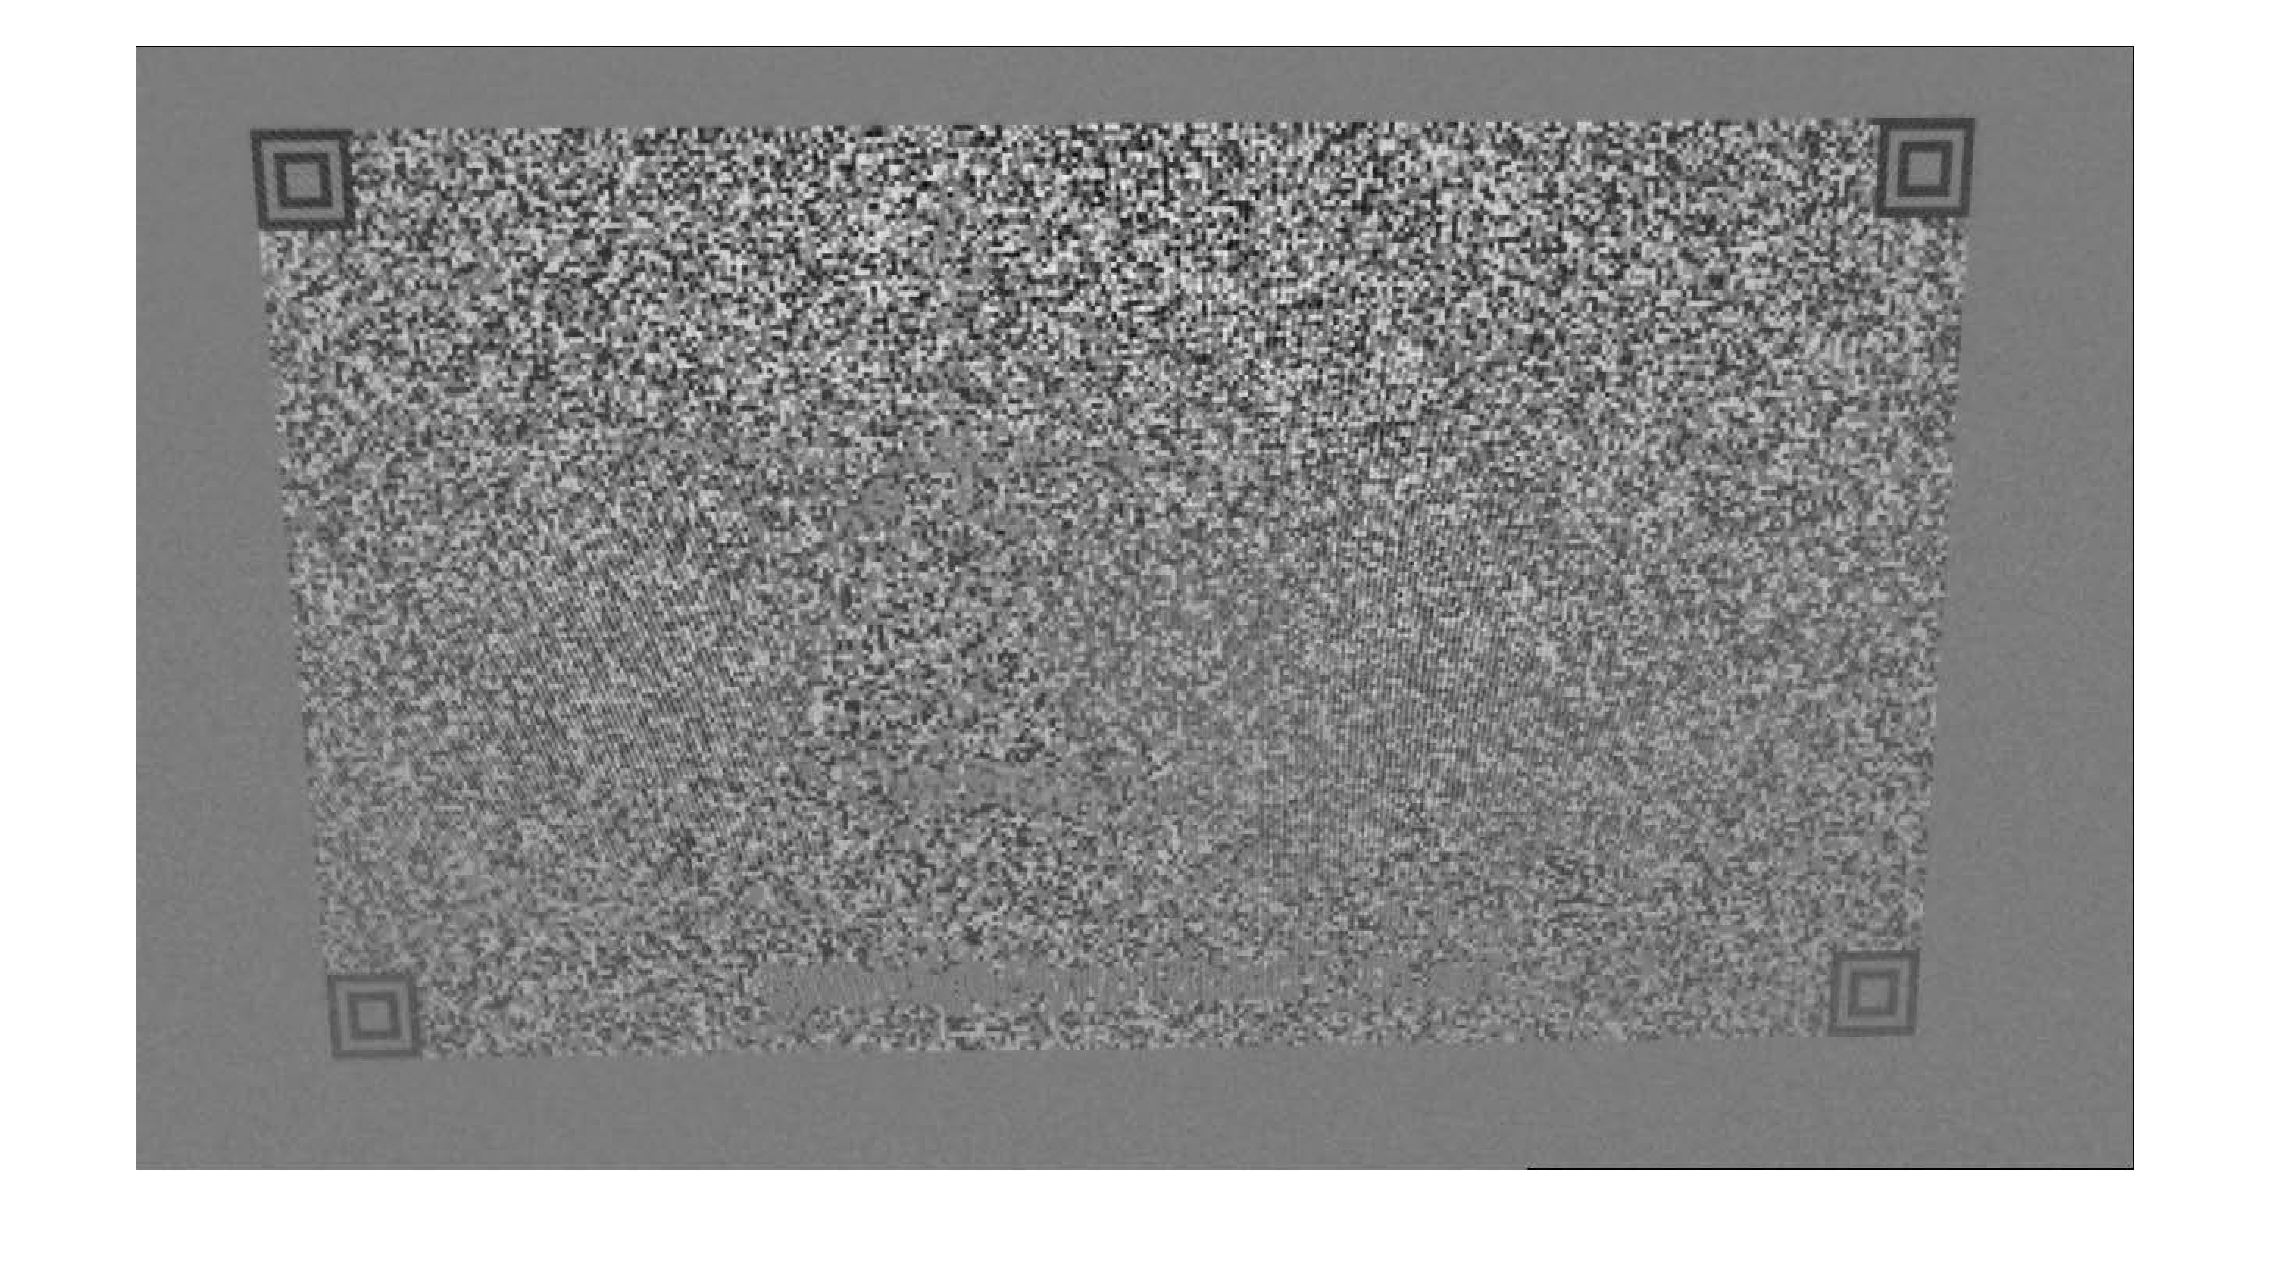
\includegraphics[scale=0.15]{images/3_Ersteverfahren/Differenzbild/2weis.pdf}& Nein & 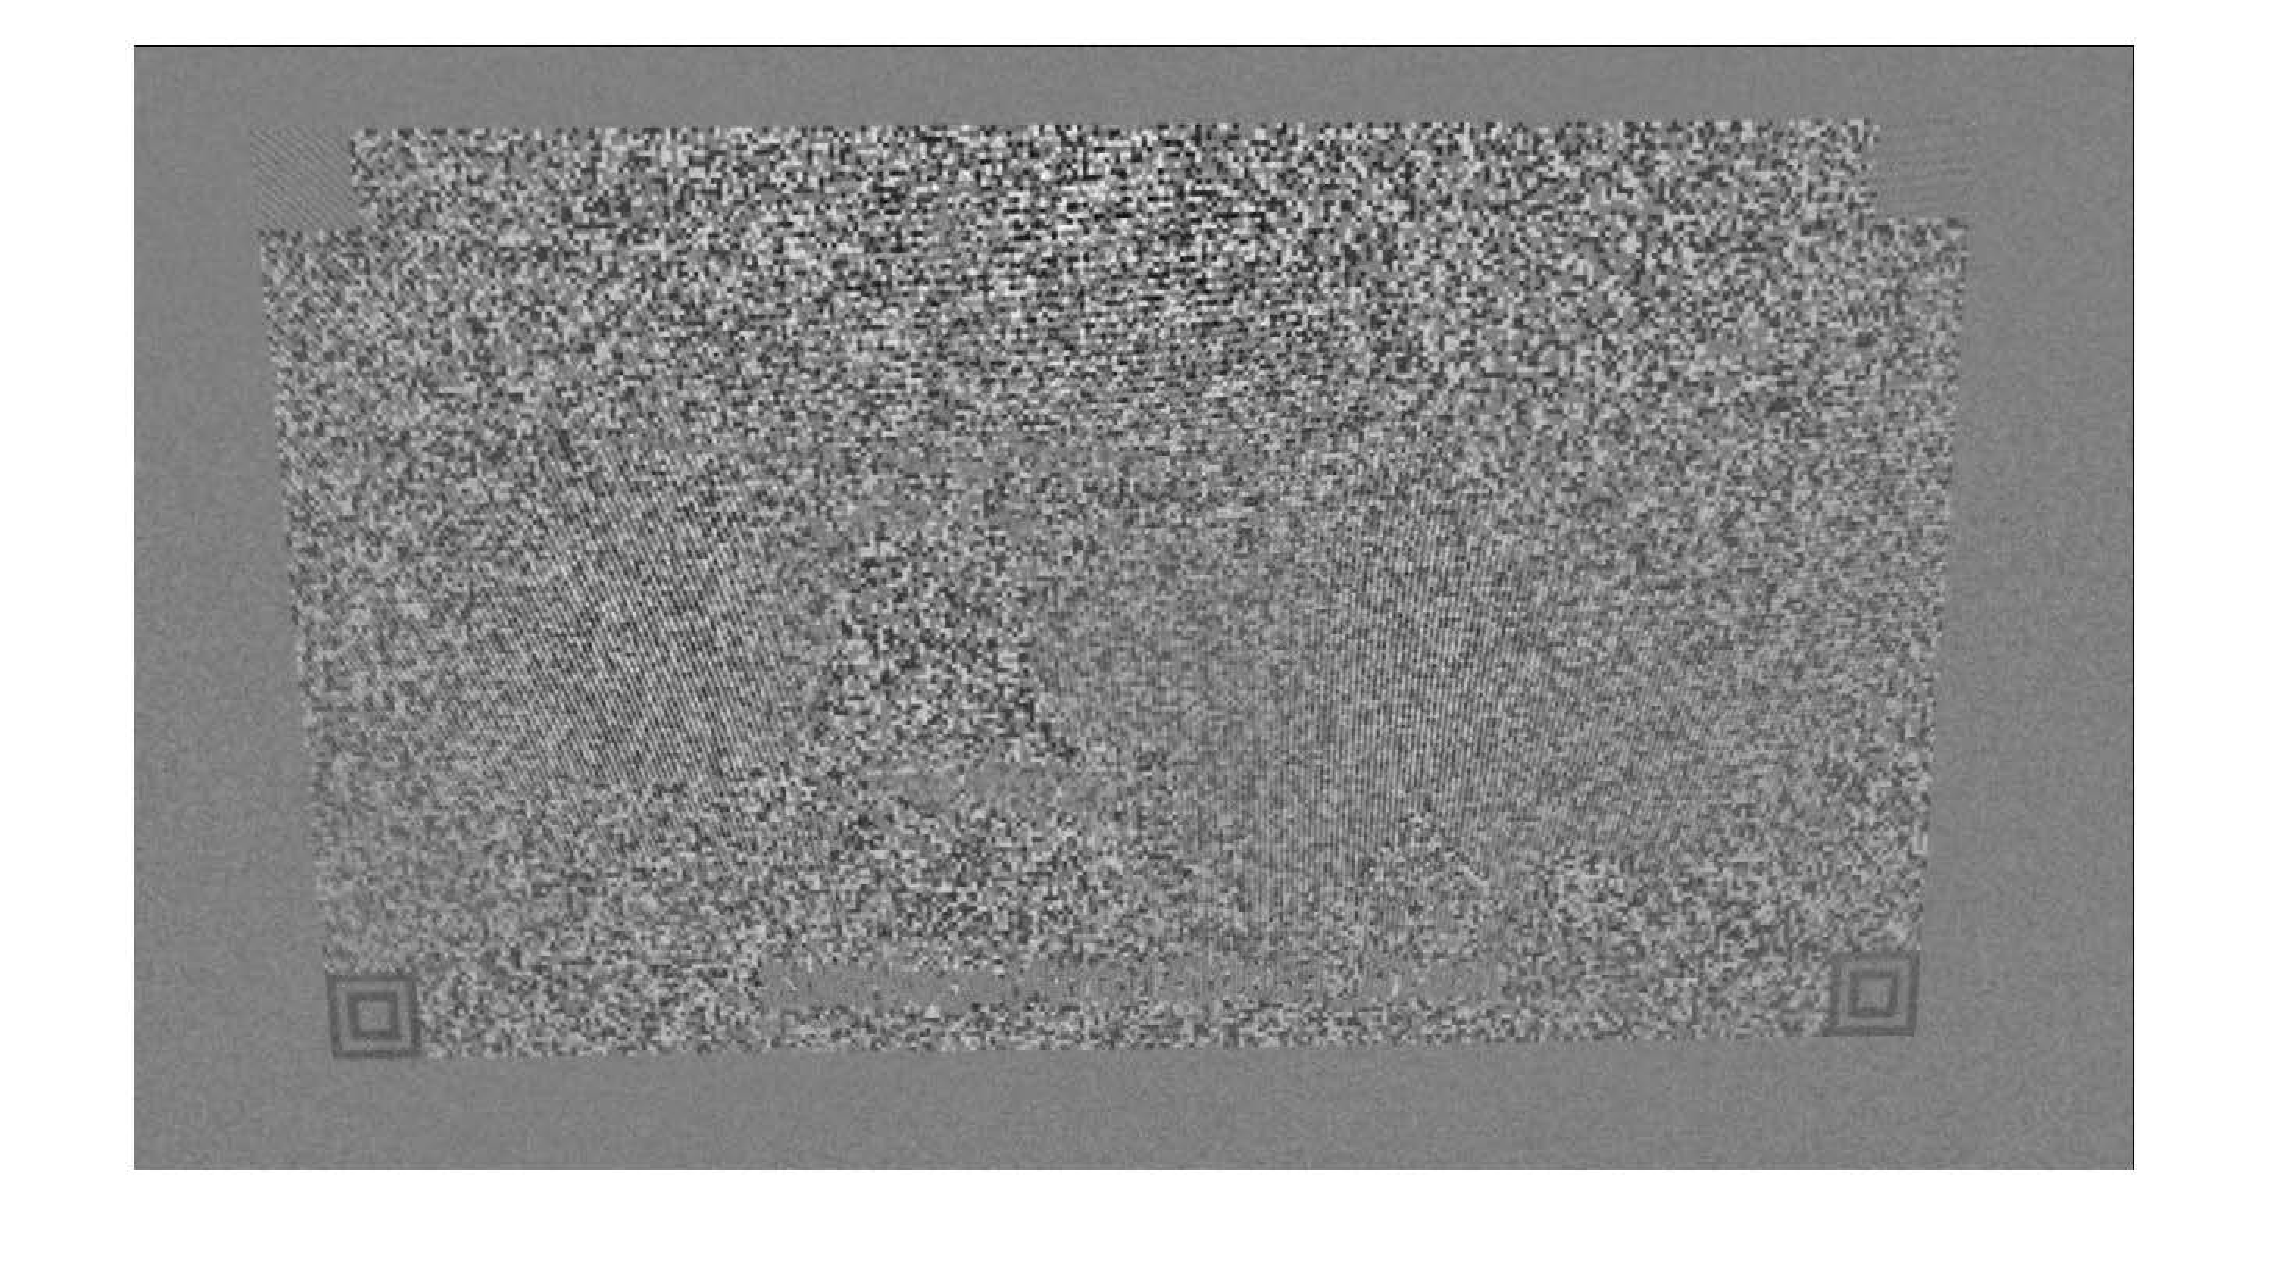
\includegraphics[scale=0.15]{images/3_Ersteverfahren/Differenzbild/3halfweis.pdf}\\
	Nein & 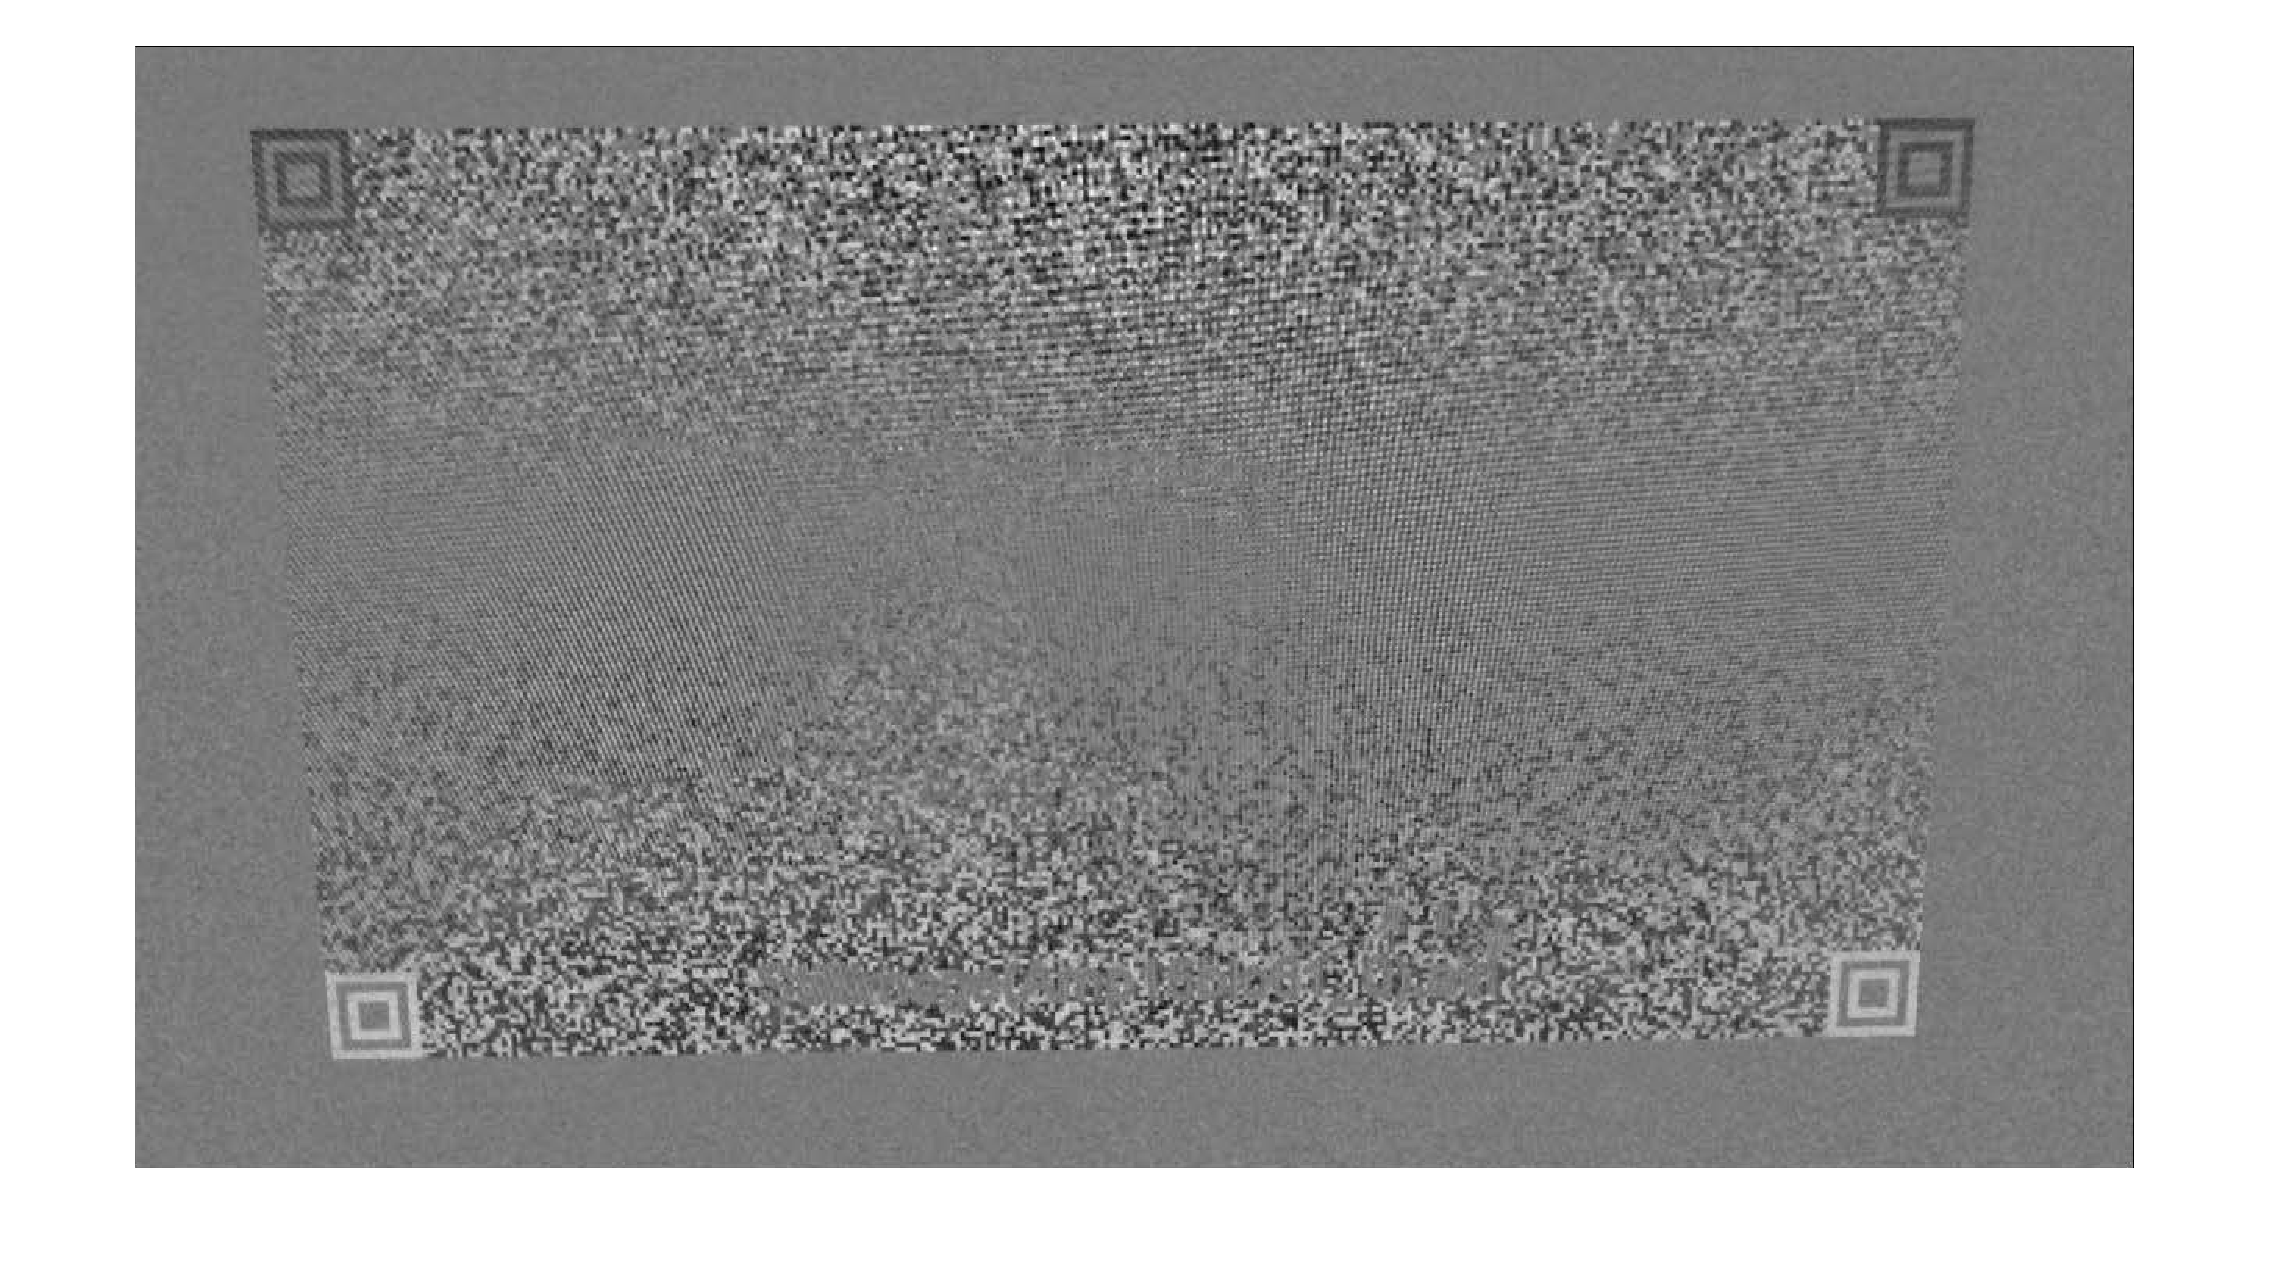
\includegraphics[scale=0.15]{images/3_Ersteverfahren/Differenzbild/4halbschwaryhalbweis.pdf}& Nein & 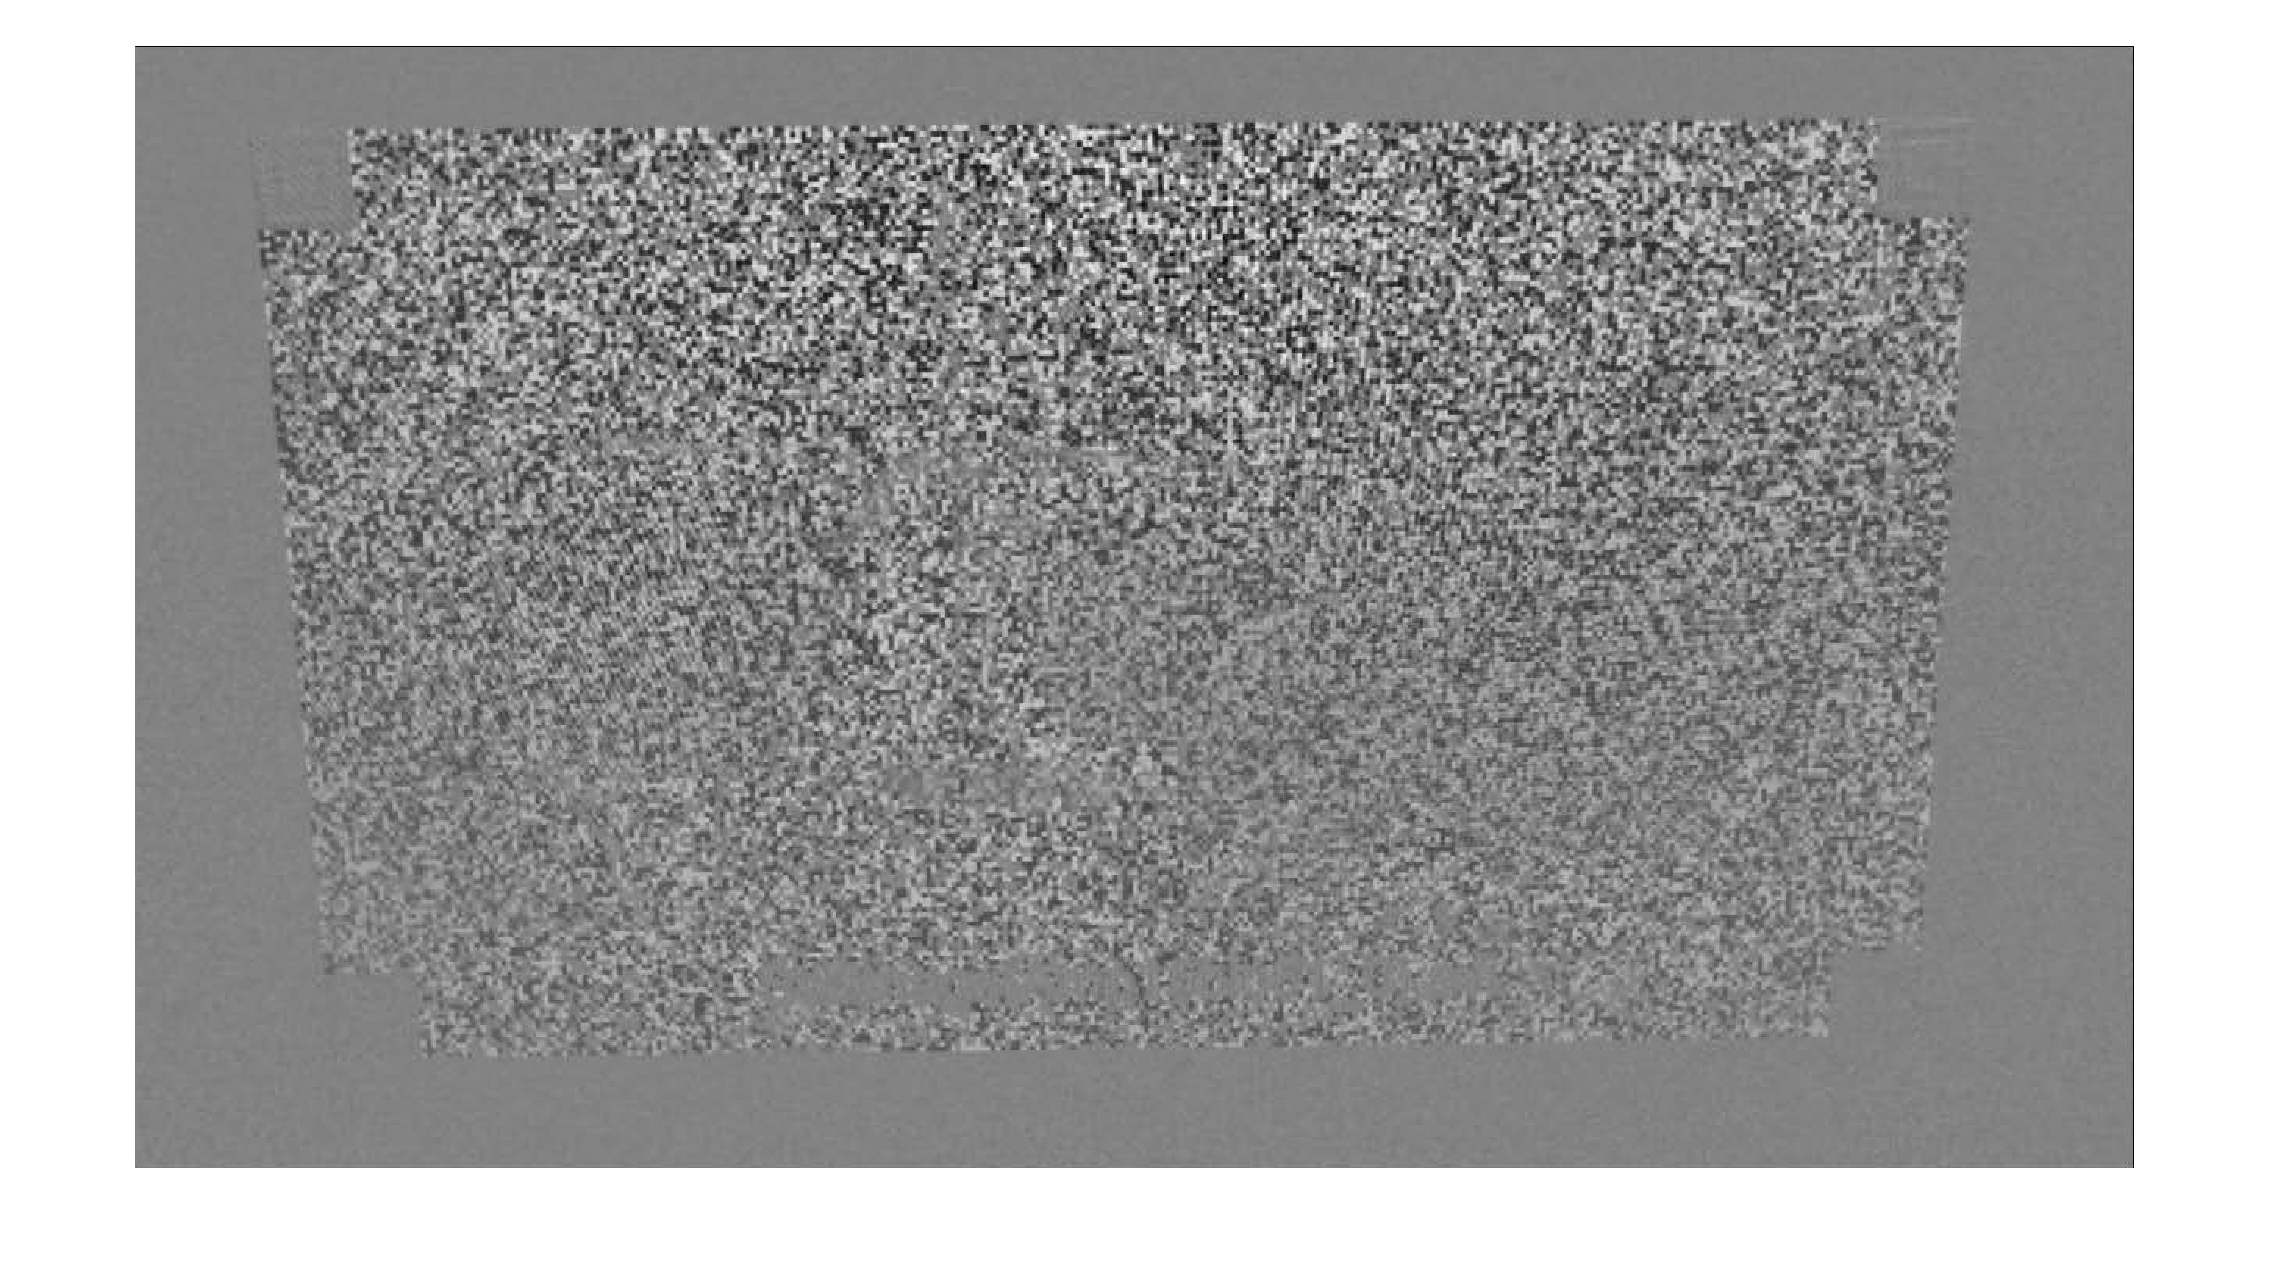
\includegraphics[scale=0.15]{images/3_Ersteverfahren/Differenzbild/5aufheben.pdf}\\

	\bottomrule
	\end{tabular}
\end{table} 


Offensichtlich ist die direkte Verwendung dieser Differenzbilder ein kniffliges Problem für die nächste Detektion. Um dieses Problem zu lösen, wurde ein Algorithmus zur Optimierung der Differenzbilder entwickelt.

Der Struktur eines QR Musters zeigt in Formel 4.29. Die äußerste $``1"$ Schicht ist hier eine Trennmuster und die Zentralbereich bedeutet das QR Muster. Aufgrund der Modulationseigenschaften des \gls{david} Systems wird nur die Pixelwert des Punkts mit Element $``1"$ nach Modulation offensichtlich verändert. Im Vergleich dazu werden die Pixelwert des Punkts mit Element $``0"$ nur klein verändert. Deswegen durch eine Absolutwertoperation, werden die QR Muster als Schwarz-Weiß-Schwarz-Weiß-Schwarz Ordnung darstellt. Dies ist die erwartende Modellstruktur, die in nächster Schritt operieren werden. Der detailliertes Operieren wird in Abschnitt "QR Muster Detektion" gegeben.

\begin{equation}
QR_{base} = \begin{bmatrix}
    1 &1 &1 &1 &1 &1 &1 &1 &1 \\
    1 &0 &0 &0 &0 &0 &0 &0 &1 \\
    1 &0 &1 &1 &1 &1 &1 &0 &1 \\ 
    1 &0 &1 &0 &0 &0 &1 &0 &1 \\ 
    1 &0 &1 &0 &0 &0 &1 &0 &1 \\ 
    1 &0 &1 &0 &0 &0 &1 &0 &1 \\ 
    1 &0 &1 &1 &1 &1 &1 &0 &1 \\ 
    1 &0 &0 &0 &0 &0 &0 &0 &1 \\ 
    1 &1 &1 &1 &1 &1 &1 &1 &1 \\ 
\end{bmatrix}
\end{equation}

Als nächstes werden ein Begriff $``Energie"$ vorstellen. Die auf numerischer Ebene bedeutet den Mittelwert des quadrierten Pixels des Bildes. Es ist bekannt sein, dass aufgrund der Subtraktion die Pixelwerte in das Gebiet, welches rund um die Modulationsbereich legt, gegeneinander aufgehoben werden. Deswegen in dieses Gebiet die Pixelwerte werden nur von Rausch beeinflusst und sehr klein sein werden. Im Vergleich dazu beträgt die Pixelwerte im Modulationbereich ein relativ größer Wert $\pm2A$, hier A beutet die Modulationsamplitude des Systems. Überlegen die Einfluss von Zeitsynchronisation, indem die Pixelwerte in einigem Teile der Modulationsbereich werden aufgrund Synchronisation auch ausgeglichen, nämlich die $``Energie"$ aufgehoben werden. Dann nehmen eine Regelmäßigkeit, die Größe der $``Energie"$ hängt hauptsächlich von die Pixelwerte im Modulationsbereich. Je größer die Pixelwerte sind, je höher der $``Energie"$ des Bildes ist, und je klarer das QR Muster werden. Gemäß dieser Regel berechnen die $``Energie"$ jedes Differenzbildes und anordnen in absteigender Reihenfolge. Um die folgende Detektion zu vereinfachen, fügen die ersten paar Bilder hinzu und erhalten einen zu detektierende Bilder. Die Praxis hat bewiesen, dass es ausreicht, die ersten drei Bilder zu nehmen.

Die Formel der $``Energie"$ wird in Gleichung 4.30 darstellt. Hier m,n repräsentiert die Anzahl der Zeilen und Spalten der Matrix. $diff(i,j)$ bedeutet die Pixelwert des Punkts in der m-ten Zeile die n-te Spalte der Matrix.

\begin{equation}
Energie = \frac{1}{m \times n} \sum_{i=1}^m \sum_{j=1}^n diff^2(i,j) 
\end{equation}

Als folgend legt die detailliert Schritt dieses Algorithmus-

\begin{enumerate}
	\item Wähle zwei beliebige Bilder aus und subtrahiere, um Differenzbild zu enthalten.
	\item Nehmen eine Absolutoperation für jedes Differenzbild und berechnen dessen Energie. 
	\item Sortiere in absteigender Reihenfolge und nehmen die erste 3 Differenzbildern.
	\item Addieren diese 3 Differenzbildern, um eine detektierend Bild zu erhalten.
\end{enumerate}

Das Flussdiagramm wird in Abbildung \ref{fig:DifferenzbildFlussigdiagramm} gezeigt.
\begin{figure}[H]
 \centering 
 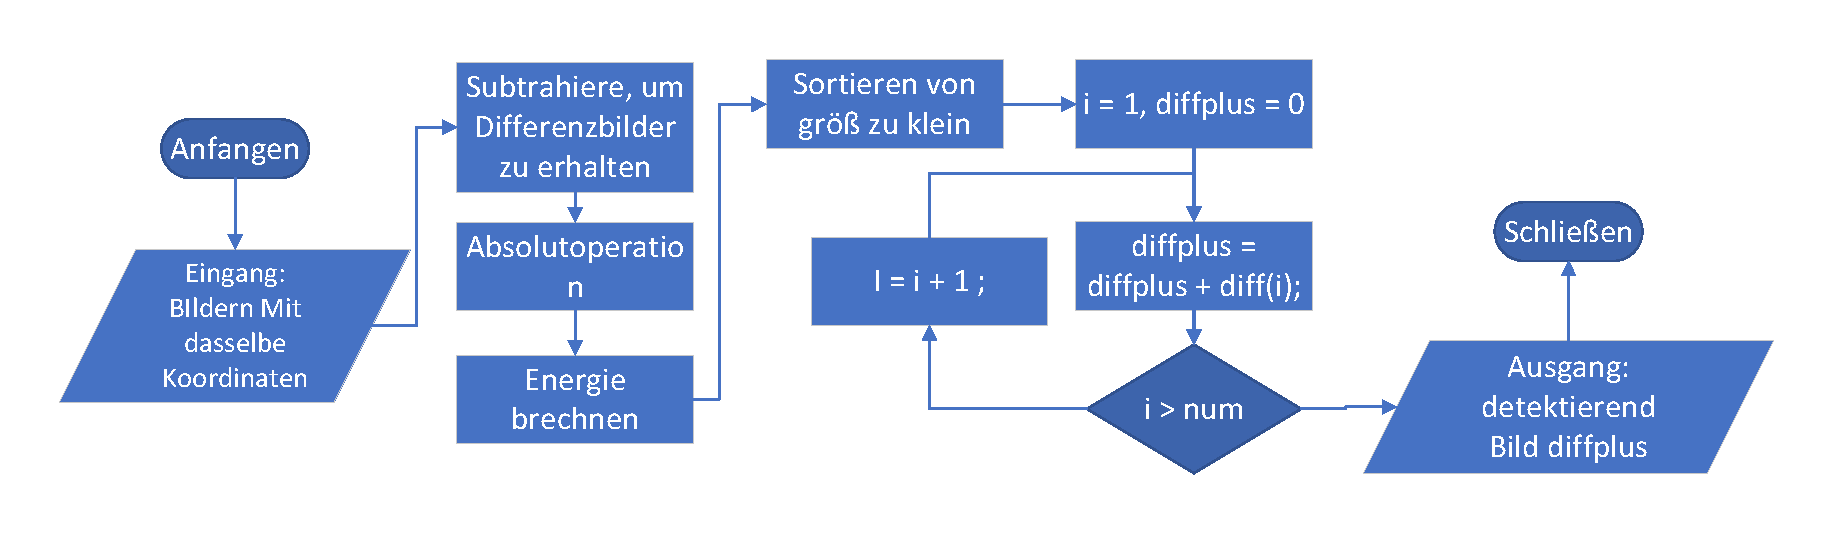
\includegraphics[keepaspectratio,width=1.1\textwidth]{images/3_Ersteverfahren/Differenzbild/Differenzbildflussigdiagramm.pdf}
 \caption{Differenzbild Flussigdiagramm}
 \label{fig:DifferenzbildFlussigdiagramm}
\end{figure} 

Eine Beispiel für detektierendes Bild wird in Abbildung \ref{fig:EindetektierendesBild} gezeigt. Aus der Abbildung ist ersichtlich, dass der Modulationsbereich besser dargestellt ist und an den vier Eck des Bereichs ein eindeutiges QR Muster vorhanden ist. Als nächstes werden die Bildverarbeitung einführen.

\begin{figure}[H]
 \centering 
 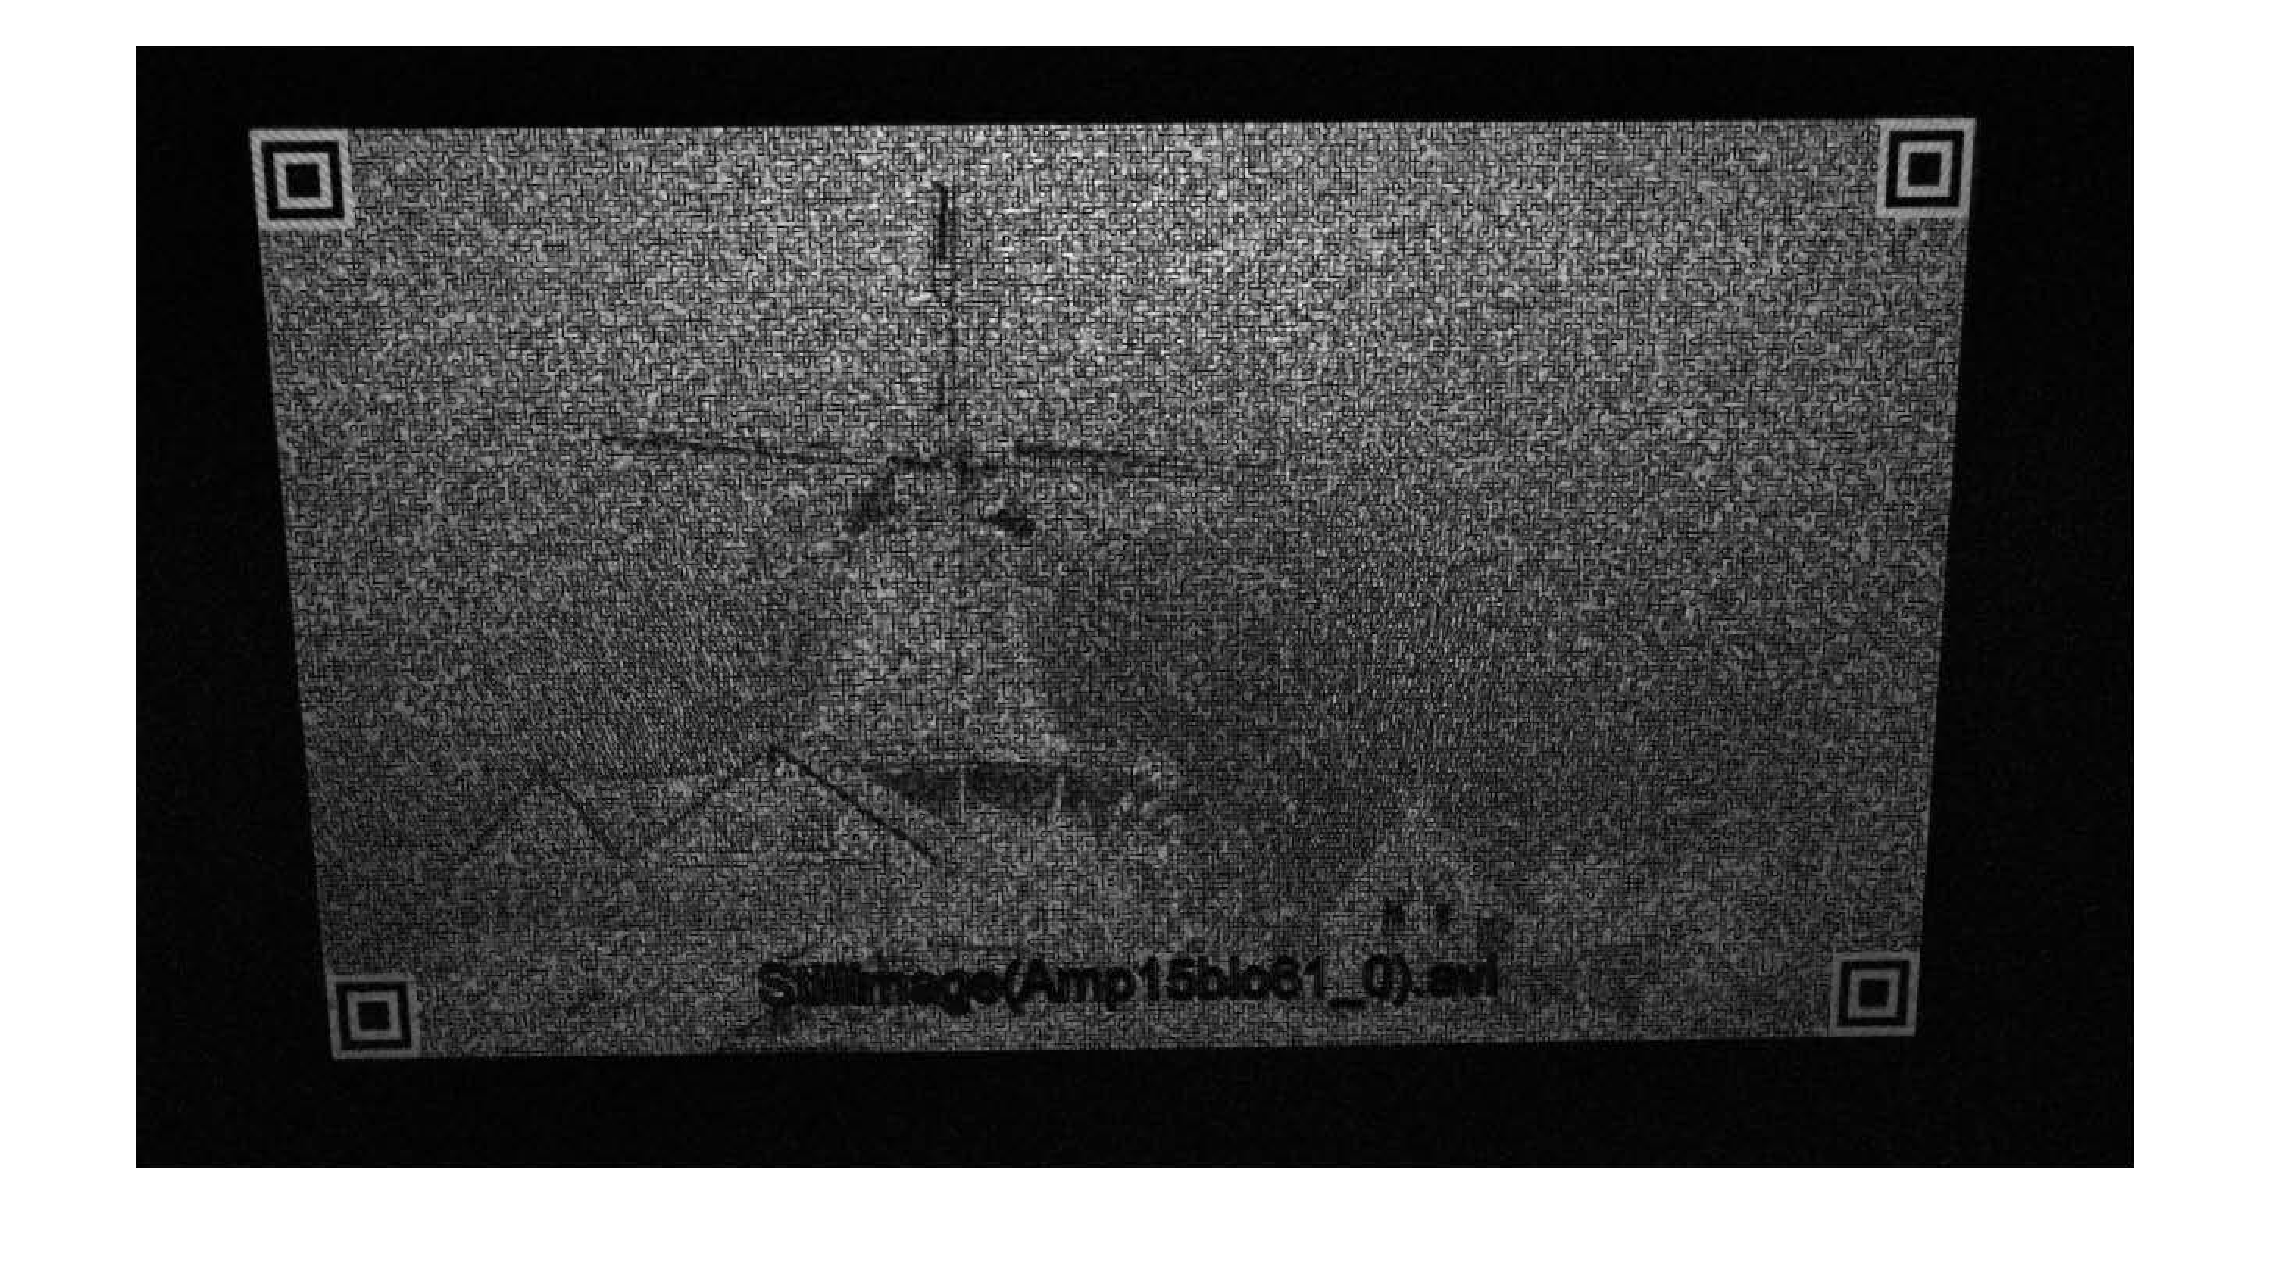
\includegraphics[keepaspectratio,width=0.8\textwidth]{images/3_Ersteverfahren/Differenzbild/diffplus.pdf}
 \caption{Ein detektierendes Bild}
 \label{fig:EindetektierendesBild}
\end{figure} 


\section{Bildverarbeitung} 
Durch die Differnzbild Optimierung, wird ein detektierendes Bild enthältet. Es ist noch ein Graustufenbild und muss noch einige Bildverarbeitung nehmen. Dadurch können kleine Punkte und Lücken, die durch Rauschen und Fehler verursacht werden, entfernt werden, um die nachfolgende Detektion zu erleichtern. Der detailliert Inhalt der Bildverarbeitung wurde in der anderen Methode eingeführt, hier ist nur eine kurze Beschreibung der verwendeten Funktionen in Matlab. 

\textbf{Bild Binarisierung}

Für die Schwellenwertbildung und das Erstellen eines Binärbildes wurde eine Funktion namens "imbinarize" verwenden. Diese Funktion erhält das Bild und verwendet ein anpassungsfähige Schwellwert, um das Schwarz-Weiß-Bild zurückzugeben. Das ist genug für QR-Pattern Detktion, weil es nur dunkle und helle Module enthält, die binär 1 bzw. 0 sind. 

\textbf{Medianfilter}

Der Grund für das Median-Filtern ist, dass manchmal beim Prozess Binarisierung aus einem Bild die Muster wie Salz- und Pfeffergeräusche erzeugt werden können. Um diesen Fehler zu vermeiden, ist Median Filterung eine leistungsfähig Methode. Das Skript ist so einfach wie medfilt2(img). Zur Verbesserung der Ergebnisse kann natürlich die verschiedenen Fenstergrößen für die Matlab-Funktion verwenden.

\textbf{Morphologie}

Mit öffnenden und schließenden Filtern können die Lücken zwischen Blöcken und die kleine Punkte von Rausch stark reduziert werden, was das resultierende binär Bild zu einer guten Schätzung des QR-Pattern macht. 

\section{QR Musters Detektion} 

Nach Bildverarbeitung wird nun die QR Musters Detektion ausgeführt. Die Ziel einer QR Musters Detektion ist die Zentrum des Musters im Bild zu lokalisieren und dadurch die Bild zu rekonstruieren. Abbildung \ref{fig:QRPattern} zeigt eine geometrische Struktur des QR Musters. An jedem Ecke der Modulartionsbereiche gibt es eine solche QR Muster.

\begin{figure}[H]
 \centering 
 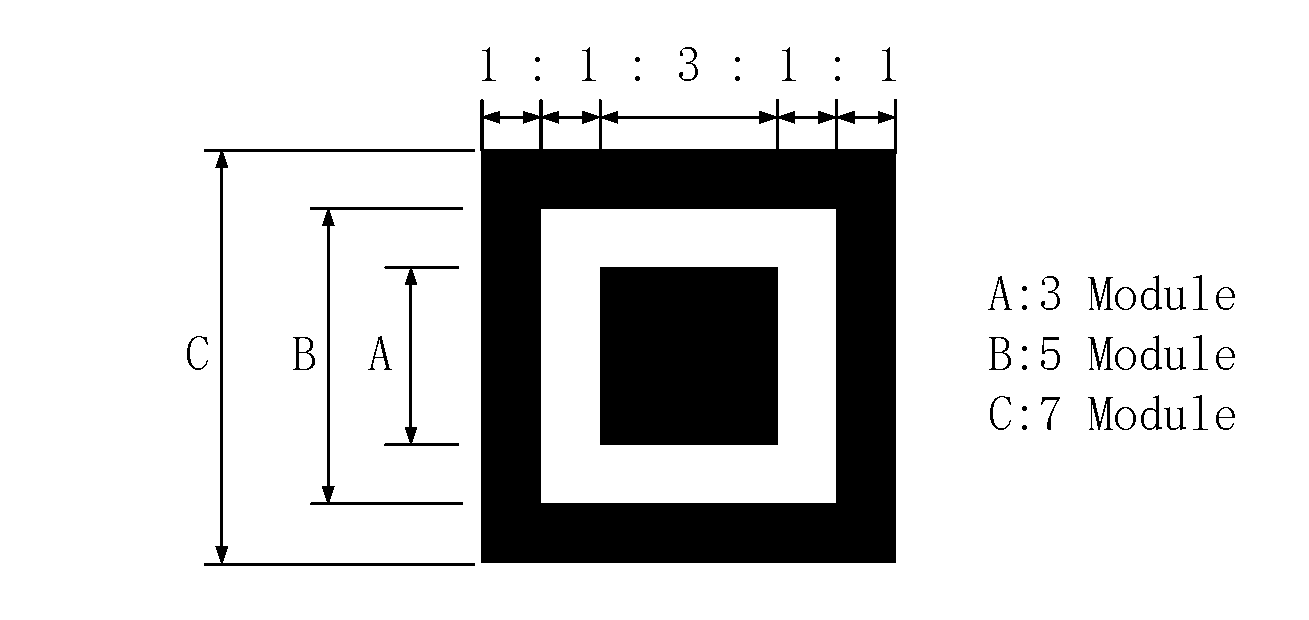
\includegraphics[keepaspectratio,width=0.9\textwidth]{images/3_Ersteverfahren/QRMuster/QRPattern.pdf}
 \caption{QR Pattern}
 \label{fig:QRPattern}
\end{figure}

Aus der geometrischen Sicht kann jedes Muster als drei konzentrische Quadrate betrachtet werden und besteht aus eine schwarzen (dunklen) $7 \times 7$ Modulen, eine weißen (hellen) $5 \times 5$ Modulen und schließlich eine dunklen $3 \times 3$ Modulen. Von Kenntnisse der Geometrie können bekannt sein, in jeder Richtung das Breiteverhältnis der alternativen Schwarz- und Weißmodul in einem Muster eine Bieziehnung $1:1:3:1:1$ beträgt, wie es in Abbildung \ref{fig:QRPatternRatio} zeigt. Diese wichtige Eigenschaft hilft uns, die Lokalität der QR Muster zu finden. In der Praxis rund um die Muster gibt es noch ein Trennmuster, das ein Funktionsmuster mit aller weißen (hellen) Module(Breit ein Modul). Es spielt eine Rolle als eine Grenze zwischen den Mustern und dem Datenbereich, um die Verwechslungen zwischen Muster und Daten zu vermeiden.
 
 \begin{figure}[H]
 \centering 
 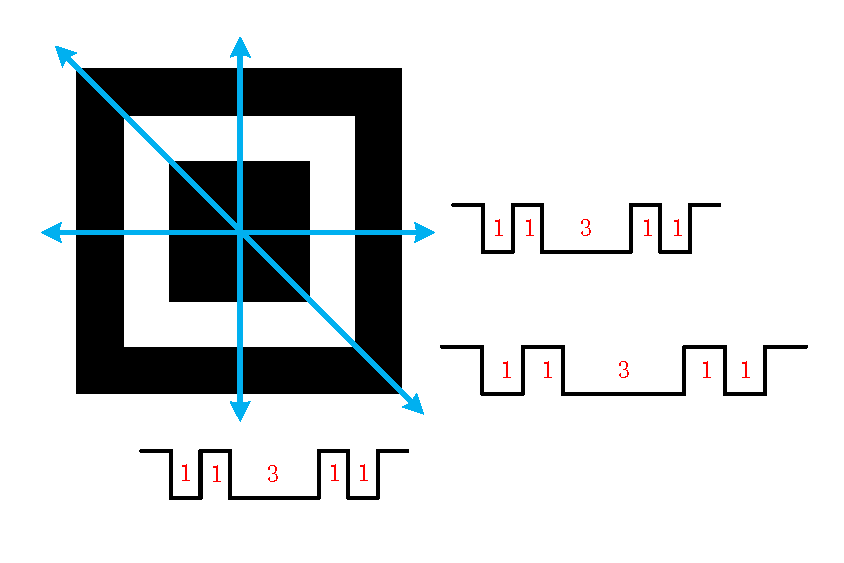
\includegraphics[keepaspectratio,width=0.7\textwidth]{images/3_Ersteverfahren/QRMuster/QP_Patternratio.pdf}
 \caption{QR Pattern Ratio}
 \label{fig:QRPatternRatio}
\end{figure}

Als nächstes werden die detaillierten Schritte der Detektion eingeführt und es wird mit Funktion "detectFIP" in Matlab implementiert.

\textbf{Schritt 1:}

Zuerst überlegen die größe Berechnungsaufwand für die Analysen des ganzen  Bilds, teilen einige kleine Bereiche auf, die QR Muster enthalten können.

\textbf{Schritt 2:}

Scannen jede Zeile dieses kleinen Bereiches und speichern die Länge der Schwarz und Weiß Module in eine fünf Element Vektor. Die Länge der Module heißt die Anzahl aufeinanderfolgende Pixel in einer Zeile mit die gleiche Farbe. Speicherreihenfolge in diesem Vektor ist laut Schwarz-Weiß-Schwarz-Weiß-Schwarz. Es sollte hier angemerkt werden, dass das erste Element des Vektors die Anzahl der schwarzen Module enthält. 

\textbf{Schritt 3:}

Immer wenn das fünfte Element des Vektors gezählt wird, nehmen die fünf Elemente und ein Urteil machen, ob die Beziehung der Zählungen nahe genug an den $1:1:3:1:1$ Verhältnissen ist. Wenn die Bedingung erfüllt ist, gehen zum nächsten Schritt. Dagegen verschieben den Vektor um zwei nach links und werfen die ersten und zweiten Elemente des Vektors weg. AnschliSeßen gehen zurück zu Schritt 2, um weiter Scannen und Zählen zu beginnen.                

\textbf{Schritt 4:}

Verarbeiten die Elemente vom Vektor, um das ungefähre horizontale Zentrum zu erhalten. Mache eine Kreuzprüfung an diesem Punkt, welche besteht aus den Schritten 2 und 3, der Unterschied dazwichen wird der horizontale Scan durch einen vertikalen Scan ersetzt. Anschließen machen ein Urteil, ob eine vertikale Zentrum gefunden ist. Wenn Ja bestimmt, machen eine Kreuz-Kreuzprüfung mit horizontale Scan, um die Ergebnis zu optimieren. Dies wird hauptsächlich benötigt, um die reale horizontale Mitte des Musters in  extremer Schräglage Fällen zu lokalisieren. Speichern der potenzielle Zetrum, danach leeren die Elemente des Vektors und wieder zu zweiten Schritt, um einen neuen Scan machen. Ansonsten verschieben den Vektor um zwei nach links und werfen die ersten und zweiten Elemente des Vektors weg. Gehen zurück zu Schritt 2, um weiter Scannen und Zählen zu beginnen.                

\textbf{Schritt 5:}

Verarbeiten die Ausgabe des vorherigen Schritts, falls es nicht nur eine potentiell Muster Zentrum gefunden, nutzen einen "selectBestPattern", um die beste zu auswählen. Es sollte angemerkt werden, dass wenn die mögliche Muster nach dem Ende der Erkundung nicht gefunden wird, ein spezielle Signal zurückgegeben wird und die System zu Schritt Differenzbild Optimierung zurückkehren wird. Die Operation besteht darin, der ursprünglichen Bild, die aus drei Differenzbild besteht, ein mehre Differenzbild hinzuzufügen.
                       
\textbf{Schritt 6:}

Durch die gefunden Muster Zentren, machen eine projective Transformation, un die Ecke des Bildes zu bestimmen.


Die folgende Abbildung \ref{fig:FlussdiagrammQRMuster} zeigt die Flussdiagramm einer Detektion für QR Muster.

\begin{figure}[htb]
 \centering 
 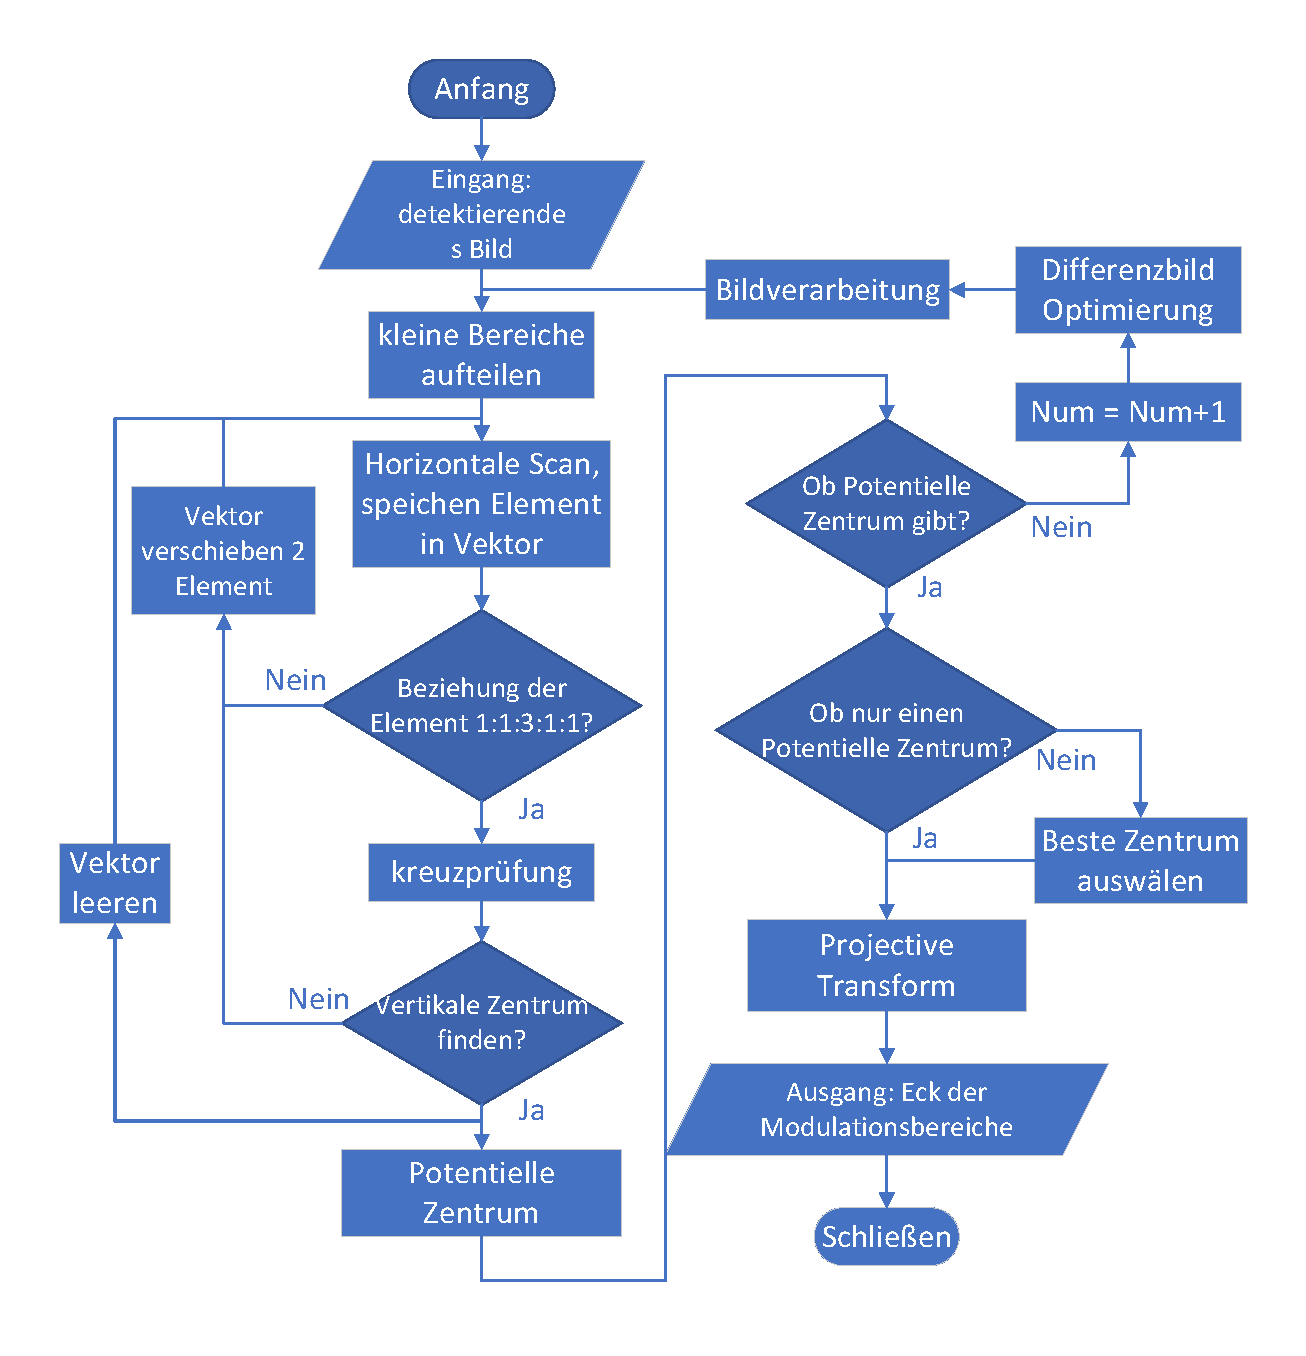
\includegraphics[keepaspectratio,width=1.0\textwidth]{images/3_Ersteverfahren/QRMuster/QR_flussdiagramm.pdf}
 \caption{Flussdiagramm der QR Muster Detektion}
 \label{fig:FlussdiagrammQRMuster}
\end{figure}

Einige Beipiel für QR Muster Detektion zeigt in Abbildung:
